%\documentclass[12pt]{scrreprt}
\documentclass[12pt]{report}

% language may be romanian or english (default is english)
% type may be bachelor or master (default is bachelor)
\usepackage[language=english, type=bachelor]{style}

% let long URLs (bibliography, footnotes) break at any character
% instead of overflowing the text block
\usepackage{xurl}

% breakable inline code for file paths and long identifiers: same
% xurl line-breaking as URLs, no hyphens inserted at the breaks
\DeclareUrlCommand\code{\urlstyle{tt}}

%controlling the appearance of your headers and footers
\usepackage{fancyhdr}
\pagestyle{fancy}
\lhead{}
\chead{}
\renewcommand{\headrulewidth}{0.2pt}
\renewcommand{\footrulewidth}{0.2pt}

\usepackage{listings}
\usepackage{xcolor}
\usepackage{graphicx}
\usepackage{amsmath}
\usepackage{amssymb}
\usepackage{tikz}
\usetikzlibrary{positioning, arrows.meta, shapes.geometric, fit, backgrounds}
\usepackage{booktabs}
\usepackage{pgfplots}
\pgfplotsset{compat=1.18}
\pgfplotsset{table/search path={figures/}}
\usepackage[newfloat]{minted}
\setminted{
  fontsize=\footnotesize,
  frame=single,
  framesep=4pt,
  breaklines=true,
  tabsize=2,
  bgcolor=gray!3
}
\usepackage[most]{tcolorbox}
\newtcolorbox{calloutbox}[1]{
  colback=blue!3, colframe=blue!50!black, fonttitle=\bfseries,
  title=#1, boxrule=0.6pt, arc=2pt, left=6pt, right=6pt,
  top=4pt, bottom=4pt
}

% give TeX extra stretch on overfull lines so inline code spans
% near the right margin do not poke past the text block.
\setlength{\emergencystretch}{3em}

% words TeX keeps breaking at awkward positions in body text — keep them whole
\hyphenation{deliberately discloses}
\graphicspath{{figures/}}

\lstset{
  basicstyle=\ttfamily\small,
  keywordstyle=\color{blue}\bfseries,
  commentstyle=\color{gray},
  stringstyle=\color{red!70!black},
  breaklines=true,
  frame=single,
  captionpos=b,
  tabsize=2
}

\begin{document}

\specialization{Computer Science}
\title{An Architectural Proposal for a Hybrid LLM-Augmented
Shopping Recommender with Grounded Output}
\author{Mihai-Dan Crisan}
\supervisor{PhD Assoc. Professor Adriana Guran}

\maketitle

% Romanian-language title page (mirrors the English one above, hand-built
% because the style package only emits one title page per build).
\begin{titlepage}
  \begin{center}
    {\Large\textbf{
      UNIVERSITATEA BABE\c S-BOLYAI CLUJ-NAPOCA \\
      FACULTATEA DE MATEMATIC\u A \c SI INFORMATIC\u A \\
      SPECIALIZAREA INFORMATIC\u A ENGLEZ\u A \\
    }}
  \end{center}

  \vspace{10em}

  \begin{center}
    {\Huge\textbf{LUCRARE DE LICEN\c T\u A}}
  \end{center}

  \vspace{3em}

  \begin{center}
    {\huge\textbf{O Propunere de Arhitectur\u a pentru un
    Sistem Hibrid de Recomandare pentru Cump\u ar\u aturi cu
    Asistent LLM \c si R\u aspunsuri Ancorate \^in Catalog}}
  \end{center}

  \vspace{10em}

  \begin{flushleft}
    {\Large\textbf{Conduc\u ator \c stiin\c tific \\ Lect. Adriana Guran}}
  \end{flushleft}

  \vspace{3em}

  \begin{flushright}
    {\Large\textit{Absolvent \\ Mihai-Dan Crisan}}
  \end{flushright}

  \vfill

  \begin{center}
    {\Large{\the\year}}
  \end{center}
\end{titlepage}

\newpage
\pagenumbering{roman}

\textbf{\Large ABSTRACT}
\vspace{0.5cm}
\hrule
\vspace{0.5cm}

This thesis studies how large language models can be brought into e-commerce recommendation: the classical recommender algorithms, the ways production AI shopping assistants fail, and the grounding techniques that prevent those failures. It then builds and evaluates a prototype that puts the study into practice: a hybrid LLM-augmented shopping recommender with grounded output. The work is motivated by documented failures in the largest production AI shopping assistant. Amazon's Rufus is credited with roughly \$12 billion of incremental revenue in 2025, yet independent investigations report 32\% recommendation accuracy, 28\% price hallucination, 83\% self-serving recommendations, and routine fabrication of review themes. The thesis argues that these failures are not built into the AI-shopping problem but follow from specific integration choices, and that a different system can make those choices differently.

The prototype combines three structural decisions. First, a reactive-first interaction model: behavior signals prepare context, but the user always starts an LLM call. Second, a two-stage recommendation pipeline: classical algorithms generate candidates, and the LLM only re-ranks and explains. Third, a hydration-over-generation principle: the LLM emits product identifiers, the client renders live catalog data, and an output-validation layer verifies every cited identifier, strips factual claims from free text, and checks review themes against the source corpus.

A custom evaluation harness scores grounded quality, latency, and cost across an eight-configuration sweep. It combines deterministic shopping-domain scorers with cross-family LLM-judge rubrics. The harness produces cost-quality and latency-quality tradeoff curves plus a composite ranking, so the shipped configuration is chosen on measured evidence rather than vendor defaults or intuition. An ungrounded baseline with the same model and no tool access validates the architecture itself: it makes twice as many specific claims, two thirds of them fail the database check, and the LLM judges still score it higher, which shows why grounding must be checked programmatically.

\tableofcontents

\newpage
\pagenumbering{arabic}

\chapter{Introduction}
\label{chap:intro}

\section{Context and Motivation}
\label{sec:intro-context}

Online retail has outgrown what any one shopper can browse. A
single category page on a large marketplace lists thousands of
substitutes, and shoppers spend a lot of time browsing, comparing,
and validating products before they buy. Recommender systems
narrow the search space using signals like co-purchase frequency,
content similarity over product attributes, and ranking models
trained on historical
interactions~\cite{ComprehensiveRecSys2024, LLM4Rec2025}. These
methods are well studied, fast, and widely deployed. They share
one limitation that hits the user directly: the output is opaque.
A shopper who sees a ``frequently bought together'' or
``similar items'' panel is not told why those products were
chosen.

Large language models reopen the explanation problem. An LLM can
write natural-language rationales, summarize customer reviews,
and surface tradeoffs between similar
products~\cite{LLMEnhancedRecSys2024, ExplainableRecKG2024}.
Putting an LLM into a shopping flow brings new risks, though.
Amazon Rufus is the most visible case in production. The system
serves over 300 million users and is credited with roughly
\$12 billion in incremental sales~\cite{RufusRevenue2025}.
Despite that scale, independent studies report a 32\% accuracy
rate for picking the right product, a 28\% price hallucination
rate, and an 83\% bias toward Amazon-owned
products~\cite{RufusWrong2024,RufusConfidentlyWrong2024}.
Consumer surveys back this up. 55\% of users say they do not
trust AI chatbot product
recommendations~\cite{ConsumerDistrust2025}, and 42\% see
e-commerce AI assistants as upsell tools, not
advisors~\cite{AIUpsell2025}. HCI research adds a timing angle:
AI suggestions offered after a natural pause land better than
proactive interruptions~\cite{CHI2024Timing}.

The open question is not whether to put LLMs into e-commerce,
but how. The architecture and interaction choices that decide
whether the assistant is trusted, accurate, and welcome have not
been studied systematically at bachelor-thesis scale against a
documented production baseline.

\section{Motivation}
\label{sec:intro-motivation}

Two facts shape the design space. First, the failure modes of
production AI shopping assistants are documented, not
speculative. Hallucinated product data, fabricated review themes,
and perceived intrusiveness all show up in Rufus and in user
surveys, and they are not edge
cases~\cite{RufusWrong2024,ConsumerResistanceAI}. Second, the
timing of an AI suggestion matters. Suggestions offered after a
natural pause read as helpful. Suggestions injected during active
deliberation read as
interruption~\cite{CHI2024Timing,ProactiveReactivePersonalization}.

A reactive-first interaction model follows. The system tracks
lightweight browsing signals (dwell time on a product, scroll
depth, engagement with the reviews tab) to infer when help might
be welcome, but it never auto-fires AI advice. The user has to
engage on purpose. Behavior signals prepare context. The user
pulls.

Amazon's own product timeline backs this up. Rufus launched as a
reactive assistant. The proactive ``Help Me Decide'' surface was
added ten months later, after the reactive product had
stabilized~\cite{RufusTechnology,RufusScaling}. Reactive came
first at the scale that matters most.

The central claim of this thesis is that a hybrid architecture
combining classical recommender algorithms with a reactive,
grounded LLM advisor can answer real shopping questions without
inheriting the trust failures of production systems, and that
every model and prompt choice in such an architecture can be
backed by measured evidence rather than intuition.

\section{Objectives}
\label{sec:intro-objectives}

This thesis sets out to design, build, and evaluate a hybrid
LLM-augmented shopping recommender with grounded output that
puts the central claim above into practice.

\begin{enumerate}
  \item Design a hybrid recommendation architecture in which a
    classical layer (Jaccard co-occurrence for ``frequently
      bought together'', weighted attribute similarity for
      ``similar products'', exponential time decay for trending,
    and a switching hybrid for personalized slots) generates
    candidates under a tight latency budget, while the LLM runs
    only on candidate sets, never on the raw catalog.

  \item Implement a reactive-first interaction model driven by
    lightweight client-side behavior signals (dwell, scroll,
    viewport, review engagement). Signals prepare context and
    surface a subtle availability indicator. They do not trigger
    LLM calls.

  \item Build a review summarization flow that surfaces
    conflicting buyer opinions with counts, fixing the failure
    most criticized in comparable production systems.

  \item Build an AI-assisted comparison flow that produces a
    structured tradeoff between two or three same-category
    products instead of a single ``best product'' verdict.

  \item Enforce hydration over generation as a structural defense
    against hallucination: the LLM emits product identifiers, the
    client renders live data from the catalog, and a validation
    layer checks every cited identifier, strips factual claims
    from free text, and verifies review-summary themes against
    the source corpus.

  \item Evaluate the system with a custom LLM evaluation harness
    that backs every configuration choice (model, reasoning
    effort, step budget, prompt variant) with measured evidence
    on grounded quality, latency, and cost.
\end{enumerate}

\section{Thesis Structure}
\label{sec:intro-structure}

The rest of the document is four chapters.

Chapter~\ref{chap:background} surveys the literature: classical
recommender systems, LLM-augmented recommendation, research on
human-AI trust and proactive versus reactive assistance, behavior
signals as proxies for intent, and a focused Amazon Rufus case
study that grounds the specific failure modes this system
addresses.

Chapter~\ref{chap:foundations} is the theory chapter. It defines
the building blocks the prototype uses: similarity measures
(Jaccard, weighted attribute scoring, cosine, exponential time
decay), the two-stage retrieve-and-rerank pattern, the LLM-agent
loop with tool use and structured output, the
hydration-over-generation principle as a formal defense against
hallucination, and the evaluation metrics used to compare
configurations.

Chapter~\ref{chap:system} documents the prototype. It opens with
the requirements and the overall architecture, then walks
through the data layer, the classical recommendation engine, the
behavior tracking and readiness pipeline, the LLM advisor with
its tools and prompt, the review summarization batch flow, the
AI-assisted comparison surface, the output validation pipeline,
and the frontend. The chapter closes with the evaluation harness
and the measured results across a nine-configuration sweep,
including pareto fronts on cost-quality and latency-quality and
a composite ranking that justifies the shipped configuration.

Chapter~\ref{chap:conclusions} summarizes what the prototype
demonstrates, what the measured evaluation supports, and the
limitations and directions for future work.

\chapter{Background and Related Work}
\label{chap:background}

\section{Classical Recommender Systems}
\label{sec:bg-recsys}

Three families dominate e-commerce recommendation: collaborative
filtering (with co-occurrence as its lightweight special case),
content-based filtering, and hybrids of the two. Time-decayed
popularity sits alongside them as the standard method for
trending slots. Each family is covered in detail
elsewhere~\cite{ComprehensiveRecSys2024, LLM4Rec2025}; the formal
definitions used in this thesis are in
Chapter~\ref{chap:foundations}.

\subsection{Co-Occurrence and Collaborative Filtering}
\label{subsec:bg-cooccurrence}

Item-based collaborative filtering rests on a simple pattern:
users who buy product $A$ often also buy product $B$. The core
data structure is a co-purchase matrix that counts the buyers
shared by each pair of items. A similarity score is computed
from it. Jaccard is the most common lightweight choice because
it normalizes by union and is robust to differences in product
popularity~\cite{ComprehensiveRecSys2024}. Item-based variants
win at e-commerce scale because product catalogs have more buyers
per item than items per buyer. This makes the item similarity
matrix denser and more stable. The main cost is precomputation:
production deployments compute the matrix on a schedule, not per
request.

The strengths are interpretability, no model training, and
tolerance to sparse user history. The weaknesses are blindness to
product attributes (two unrelated products that share a buyer
base still link) and the cold-start problem for new products with
no purchase history.

\subsection{Content-Based Filtering}
\label{subsec:bg-content}

Content-based filtering scores similarity using product
attributes instead of purchase signals. A typical setup defines a
feature vector over category, brand, tags, and price proximity,
then computes a weighted distance between the active product and
every other product in the catalog. The main strength is the
zero-purchase cold start: a brand-new product can be recommended
on day one because its attributes are known immediately. The main
weakness is the filter-bubble effect: recommendations reinforce
the active item's profile.

\subsection{Hybrid Recommenders and Trending}
\label{subsec:bg-hybrid}

Burke's taxonomy splits hybrid recommenders into seven patterns;
weighted, switching, and mixed are deployed most
often~\cite{Burke2002Hybrid}. A weighted hybrid combines
normalized scores from multiple algorithms into a single ranking.
A switching hybrid picks which algorithm to run per request based
on context (cold versus warm user, sparse versus rich product). A
mixed hybrid shows results from multiple algorithms side by side
without combining their scores. The prototype uses a switching
hybrid for the personalized ``recommended for you'' slot. Where
scores are combined, the prototype uses Reciprocal Rank Fusion,
which avoids normalizing scores across different algorithms by
combining ranks instead~\cite{LLM4Rec2025}.

Naive popularity over an order log favors products with long-tail
demand and penalizes products that are gaining fast. Exponential
time decay corrects this by giving recent activity more weight,
with a half-life chosen per category: short for fashion and
consumer trends, long for durable
goods~\cite{SessionRecSys2021}. The formal definition is in
Section~\ref{sec:found-similarity}.

\section{Explainable Recommendations}
\label{sec:bg-explainable}

A recommendation with a reason is a different thing from one
without. Classical systems offer pattern-level explanations
(``users who bought X also bought Y'') that are interpretable but
generic. Recent work uses LLMs to generate sentence-level
rationales conditioned on user
context~\cite{LLMEnhancedRecSys2024}. Knowledge-graph-grounded
explanations sit between the two: they draw facts from a curated
graph instead of generating freely, and their rationales contain
fewer hallucinated attributes~\cite{ExplainableRecKG2024}. An
explanation improves trust calibration: users more readily accept
correct recommendations and reject incorrect ones. The thesis
treats explanation as a first-class output of the LLM stage.

\section{Large Language Models in Recommender Systems}
\label{sec:bg-llm-recsys}

Surveys of LLM-augmented recommendation identify three roles for
an LLM in the pipeline: knowledge enhancement (the LLM acts as a
knowledge source for product attributes and user intent),
interaction (the LLM is the conversational interface to a
recommender backbone), and model enhancement (LLM-derived
features feed a downstream ranker as extra
input)~\cite{LLMEnhancedRecSys2024}. The roles differ in cost and
integration depth. Interaction is the cheapest to deploy because
it sits at the surface and needs no retraining. Model enhancement
is the most invasive because it changes the offline training
pipeline. This thesis uses roles 1 and 2: the LLM contributes
knowledge (review themes, comparison narratives, product
explanations) and interaction (the conversational advisor). It
does not retrain a ranker. The data volume of a bachelor-thesis
prototype would not support it, and the architectural lessons of
the thesis are at the integration layer, not the modeling layer.

The standard pattern for combining classical recommenders with
LLMs is a two-stage architecture: a classical candidate generator
returns a small set of products under a tight latency budget, and
an LLM reranks, explains, or summarizes that set in a second
stage~\cite{HSTU2024, ShopifyHSTU}. The pressure is cost: LLM
inference scales with context size, so feeding five candidates is
cheap at consumer scale, while feeding five thousand catalog items
is not. The pattern also separates concerns cleanly. The
classical stage owns relevance and recall over the full catalog;
the LLM stage owns explanation, conflict surfacing, and tradeoff
articulation. The prototype follows this split strictly: the
classical stage runs on the full Convex catalog, and the LLM
stage only ever sees a small candidate set, never the full
catalog.

\section{Review Summarization for Purchase Validation}
\label{sec:bg-review-summarization}

Reviews drive a large share of purchase decisions, yet most
product detail pages show them raw. AI-generated review summaries
compress that reading work into a short structured output:
themes, frequently mentioned features, and (less often) explicit
conflict callouts.

Naive summarization fails in two specific ways. First, it
averages sentiment, hiding the minority opinions that often
matter most for purchase decisions (a 38-versus-9 split
between buyers who love a product and buyers who report failure
after six months is more useful than a 4.2-star average). Second,
when prompted to produce a tidy summary, it tends to fabricate
themes that are not in the source
corpus~\cite{RufusConfidentlyWrong2024}. The second failure has
drawn the most criticism of comparable production review-summary
systems. The thesis treats theme fabrication as a hard
constraint: summaries are generated against the actual review
corpus, themes are validated against the source text before they
are stored, and conflicting opinions are surfaced explicitly
with counts.

\section{AI-Assisted Comparison as Decision Support}
\label{sec:bg-comparison}

Comparison carries the highest cognitive load of any task in a
typical purchase journey. Users compare across mixed attributes
(price, battery life, build material, warranty length, shipping
speed) where the weight of each attribute depends on personal
preferences. LLMs are well suited to laying out these tradeoffs
in natural language. Industry agrees: Shopify's analysis of
agentic shopping flows names comparison and tradeoff articulation
as two of the interactions where LLMs add the most user-perceived
value~\cite{ShopifyAgentic}. Consumer research finds 56\% of
shoppers explicitly want comparison help from AI assistants and
47\% want review summarization~\cite{DigidayAIShopping}.

The main design failure in current AI comparison features is the
``best product'' verdict: the system picks a winner, hides the
tradeoffs, and takes the choice away from the user. UX guidance
for agentic AI explicitly warns against this pattern. It
recommends a tradeoff-first layout where the system surfaces the
structured differences and lets the user weight
them~\cite{SmashingAgenticUX}. The thesis follows the
tradeoff-first pattern: comparisons present structured
differences, never a verdict.

\section{Trust and Human-AI Interaction}
\label{sec:bg-trust}

\subsection{Timing and Consumer Resistance}
\label{subsec:bg-timing}

A CHI 2024 study measured how users react to AI suggestions
delivered at different times. Suggestions offered after a natural
pause were rated significantly more helpful than suggestions
injected during active deliberation~\cite{CHI2024Timing}. Related
work in human-AI personalization makes a stronger claim: reactive
personalization preserves the user's perceived autonomy, and
perceived autonomy is one of the strongest predictors of trust in
AI systems~\cite{ProactiveReactivePersonalization}. Proactive
interventions can be welcome, but only at high-confidence moments
where the system has strong evidence the user is stuck or at
decision risk.

Market data shows consumer trust in AI shopping assistants is
low. 55\% of consumers say they do not trust AI chatbot product
recommendations~\cite{ConsumerDistrust2025}. 42\% see e-commerce
AI assistants as upsell tools, not advisors~\cite{AIUpsell2025}.
71\% of retailers have deployed conversational AI in some form,
but only 16\% of consumers use these assistants
regularly~\cite{ConsumerResistanceAI}. The gap between deployment
and usage points to structural resistance. A trustworthy AI
advisor is not a polish layer on top of a shopping system; the
trust gap is the product question.

\subsection{Behavioral Signals as Intent Indicators}
\label{subsec:bg-behavior-signals}

A long line of information retrieval work shows that lightweight
client-side signals (cursor position, dwell time, scroll depth,
hover trajectory) are reliable proxies for user
attention~\cite{SIGIR2020Cursor}. The signals are cheap to
collect and need no server-side modeling at capture time. Dwell
time deserves a note. In information retrieval, dwell predicts
engagement well: the longer a user reads, the more engaged they
are. In e-commerce, dwell still predicts engagement, but it
predicts intent-to-buy less reliably; users sometimes dwell
because they are confused, comparing across browser tabs, or
distracted~\cite{DwellTimeEngagement2022}. The thesis treats
dwell as an attention proxy, not a buying-intent proxy, and
combines it with review-tab engagement and scroll depth in a
composite readiness score.

A privacy boundary applies. The prototype aggregates raw signals
client-side and persists only summary statistics to the backend.
Raw event streams are never stored or sent off the device.

\section{Case Study: Amazon Rufus}
\label{sec:bg-rufus}

Amazon Rufus is the largest deployed AI shopping assistant by
user count and the most thoroughly studied externally. Rufus is
the reference point for this section: its architecture shows the
practical shape of a production-scale AI shopping system, and its
documented failures inform several design decisions in the
prototype.

\subsection{System Architecture and Capabilities}
\label{subsec:bg-rufus-arch}

Rufus combines three architectural patterns. A multi-model router
picks an inference model per query: simple lookups go to a fast,
cheap model; reasoning-heavy queries go to a slower, more capable
one. The output is two-stream: text is streamed as it generates,
and structured product references are hydrated client-side from
live catalog data, so the user sees the explanation and the live
product card as one coherent
response~\cite{RufusTechnology, RufusScaling}. The system plugs
into Amazon's COSMO knowledge graph, an LLM-built commonsense
graph that enriches products with implicit attributes (a
children's bicycle is also ``a gift for a 7-year-old''),
reportedly improving internal relevance metrics by
60\%~\cite{COSMO}. The integration footprint is broad: Rufus
appears on the product detail page, in search, and in the cart.
It serves over 300 million users with parallel speculative
decoding to keep latency within product
targets~\cite{RufusScaling}.

\subsection{Documented Accuracy and Trust Issues}
\label{subsec:bg-rufus-problems}

External evaluations of Rufus report four classes of failure,
stable across studies. First, recommendation accuracy: independent
measurement places Rufus at 32\% accuracy for picking the right
product for a query, far below the relevance figures Amazon
reports internally~\cite{RufusWrong2024}. Second, factual
hallucination: 28\% of Rufus responses that include a product
price quote the wrong price, an error that is especially
damaging because the user can check it in
seconds~\cite{RufusWrong2024}. Third, self-serving bias: 83\% of
Rufus's recommendations favor Amazon-owned or Amazon-branded
products over third-party alternatives, which reinforces the
perception of the assistant as an upsell
tool~\cite{RufusWrong2024}. Fourth, review summary fabrication:
Rufus has been observed to generate review themes that do not
appear in the source review corpus, the failure that has drawn
the most public criticism of the
four~\cite{RufusConfidentlyWrong2024}.

The four failure modes are not independent. They share a single
root cause: the LLM is allowed to generate factual product data
(prices, attributes, themes) from its parametric memory instead
of reading only from live catalog data and source review text.
This observation motivates the output validation and hydration
strategy in Chapter~\ref{chap:foundations}.

\subsection{Feature Evolution and Lessons}
\label{subsec:bg-rufus-lessons}

Rufus's product timeline is informative beyond the architecture.
The system launched in early 2024 as a reactive assistant: the
user opened a chat surface and the system responded. The
proactive ``Help Me Decide'' surface, where the system offers to
compare or recommend without being asked, was added about ten
months later~\cite{RufusTechnology, RufusScaling}. This order
matches the CHI 2024 timing finding above: reactive came first
because it was easier to launch without breaking user
expectations, and proactive was added piece by piece once the
system had stabilized. Public reporting credits Rufus with
roughly \$12 billion of incremental sales in
2025~\cite{RufusRevenue2025}. The thesis treats this number as a
market-sizing data point, not proof of product-market fit,
because the trust failures above leave the user-experience case
contested.

\section{Positioning of This Thesis}
\label{sec:bg-positioning}

Prior work treats classical recommendation and LLM integration
as separate problems. The questions that decide whether a real
AI shopping advisor is trustworthy (when to speak, how to ground
its answers, how to surface conflicting reviews, how to catch
hallucinations) are scattered across HCI papers, engineering
blogs, and post-mortems of shipped systems.
Table~\ref{tab:bg-positioning} compares this thesis with the
systems from this chapter on the four dimensions where it makes
its design choices: how the AI surface is triggered, where facts
come from, what is checked after generation, and what evidence
backs the configuration.

\begin{table}[ht]
  \centering
  \footnotesize
  \begin{tabular}{p{2.6cm} p{2.2cm} p{2.4cm} p{2.1cm} p{2.1cm}}
    \toprule
    System & Interaction & Grounding & Output checks &
    Config evidence \\
    \midrule
    Classical recommenders \cite{ComprehensiveRecSys2024} &
    none, fixed slots &
    catalog items by construction &
    not needed &
    offline metrics \\
    Shopify generative recs~\cite{ShopifyHSTU} &
    none, ranking only &
    catalog items by construction &
    not needed, no free text &
    A/B tests at scale \\
    KG-grounded explanations~\cite{ExplainableRecKG2024} &
    rationale text per item &
    curated knowledge graph &
    graph lookups &
    offline benchmarks \\
    Amazon Rufus~\cite{RufusTechnology} &
    chat, proactive and reactive &
    RAG over catalog and web &
    none documented &
    internal, not public \\
    This thesis &
    chat, reactive only &
    hydration from live catalog &
    three-check pipeline &
    measured eval sweep \\
    \bottomrule
  \end{tabular}
  \caption{The thesis prototype next to the related systems from
  this chapter.}
  \label{tab:bg-positioning}
\end{table}

The first three rows are safe but limited. Classical
recommenders and Shopify's generative recommender emit only
catalog items, so they cannot hallucinate, but they also cannot
explain, compare, or summarize reviews. Knowledge-graph systems
add rationale text and keep it grounded in a curated graph, at
the cost of building and maintaining that graph. Rufus has the
full conversational surface, but no documented validation layer
between the model and the user, and
Section~\ref{subsec:bg-rufus-problems} lists the failure rates
that follow.

This thesis takes the combination the table leaves open: a
conversational advisor like Rufus, with the by-construction
grounding of the item-only systems, a validation pipeline on
everything the model emits, and a measured evaluation behind
every configuration choice. The contribution is not a new
algorithm. It is an integration architecture and an honest
evaluation against documented production failures, at a scale a
bachelor thesis can defend.

\chapter{Concepts}
\label{chap:foundations}

This chapter sets out the building blocks the prototype uses.
Each section defines the concept, states the property the
prototype relies on, and leaves the implementation detail for
Chapter~\ref{chap:system}. Section~\ref{sec:found-classical}
recaps the classical recommender families.
Section~\ref{sec:found-similarity} defines the similarity
measures and the time-decay function used throughout the system.
Section~\ref{sec:found-two-stage} states the two-stage
retrieve-and-rerank pattern. Section~\ref{sec:found-agents}
describes the LLM-agent loop with tool use and structured output.
Section~\ref{sec:found-grounding} develops hydration over
generation and the post-generation validation pipeline as a
structural defense against hallucination.
Section~\ref{sec:found-eval} defines the evaluation metrics used
to compare model and prompt configurations.

\section{Classical Recommender Foundations}
\label{sec:found-classical}

The classical layer uses the three families surveyed in
Chapter~\ref{chap:background}: item-based collaborative filtering
specialized as co-occurrence, content-based filtering over
weighted product attributes, and exponentially time-decayed
popularity for trending. The personalized slot uses a switching
hybrid as defined by Burke~\cite{Burke2002Hybrid}, picking the
algorithm per request based on how deep the user's purchase
history goes. Three properties of this layer matter for what
follows: every algorithm runs on the live catalog and returns
real product identifiers (it cannot invent products), every
algorithm is deterministic given the catalog state (the candidate
set is reproducible across evaluation runs), and every algorithm
runs inside a single Convex query within a tight latency budget
(Section~\ref{sec:found-two-stage}). Together they justify
treating the classical layer as the trusted source of candidates
and the LLM as a writer over those candidates.

\section{Similarity Measures and Time Decay}
\label{sec:found-similarity}

Four formal definitions support the classical layer.

\paragraph{Jaccard similarity.} Jaccard measures how much two
sets overlap, normalized by their combined size --- the share of
elements they share. For two finite sets $A$ and $B$,
\[
  J(A, B) \;=\; \frac{|A \cap B|}{|A \cup B|},
\]
with $J(\emptyset, \emptyset) := 0$ by convention. The coefficient
is symmetric, lives in $[0, 1]$, and equals one iff $A = B$.
Applied to the buyer sets of two products $p_a, p_b$, it produces
a similarity score that is robust to popularity differences: a
product with many buyers does not automatically score high
against another just because their intersection is
large~\cite{ComprehensiveRecSys2024}. The
prototype uses Jaccard over buyer sets for the ``frequently
bought together'' slot, with a minimum-support filter requiring
$|B(p_a) \cap B(p_b)| \ge 2$ for a pair to enter the precomputed
co-occurrence index. The filter suppresses spurious links from
incidental co-purchases.

\paragraph{Weighted attribute similarity.} Two products are
compared by averaging seven small attribute comparisons, with the
heaviest weight on the simplest signal (same category) and small
equal contributions from price, rating, brand, and the
LLM-enriched fields. Formally,
\[
  \mathrm{sim}(p_a, p_b) \;=\; \sum_{i=1}^{7} w_i \cdot f_i(p_a, p_b),
\]
where each $f_i$ is one of three primitives --- an indicator
$\mathbb{1}[\cdot]$ (1 if equal, 0 otherwise), the Jaccard
coefficient $J(\cdot, \cdot)$ over a tag-set argument, or a
proximity score $\mathrm{prox}(x, y) = 1 - |x-y|/\max(x,y)$ for
numeric attributes. Table~\ref{tab:found-sim-weights} lists the
components and their weights.

\begin{table}[ht]
  \centering
  \footnotesize
  \begin{tabular}{lll}
    \toprule
    Component & Weight & Primitive \\
    \midrule
    same category   & 0.25 & indicator \\
    tag overlap     & 0.20 & Jaccard \\
    use-case overlap & 0.15 & Jaccard \\
    good-for overlap & 0.10 & Jaccard \\
    same brand      & 0.10 & indicator \\
    price proximity & 0.10 & proximity \\
    rating proximity & 0.10 & proximity \\
    \bottomrule
  \end{tabular}
  \caption{Components of the weighted attribute similarity score.
    Weights sum to 1.0; category and tag overlap dominate.}
  \label{tab:found-sim-weights}
\end{table}

The \texttt{useCases} and \texttt{goodFor} fields carry implicit
attributes (a children's bicycle is also ``a gift for a
7-year-old'') and are produced once per product during seed by a
batch LLM call modeled on the COSMO knowledge graph~\cite{COSMO}.
At query time, $\mathrm{sim}$ is pure attribute arithmetic over
the denormalized product row.

\paragraph{Cosine similarity.} Cosine treats two vectors as
directions and measures the angle between them --- values near
one mean the vectors point the same way, values near zero mean
they are orthogonal. For two vectors $u, v \in \mathbb{R}^d$,
\[
  \cos(u, v) \;=\; \frac{\langle u, v \rangle}{\|u\| \cdot \|v\|}.
\]
The prototype uses cosine over text embeddings only inside the
review-theme-fidelity scorer of Section~\ref{sec:found-eval}:
each candidate review-summary theme is embedded and compared
against the embeddings of the source reviews, and themes whose
nearest review falls below a threshold $\tau$ are rejected.
Cosine beats Euclidean distance here because embedding norms
carry no semantic content.

\paragraph{Exponential time decay.} Trending is a weighted count
of recent events where each event's contribution shrinks
exponentially as it ages, so a sale from yesterday counts more
than a sale from a month ago. For a product $p$ with event set
$E_p$, per-event weight $w(\cdot)$ (a purchase weighs more than a
view), and event age $\mathrm{age}(e)$ measured in days from now,
\[
  \mathrm{trending}(p) \;=\; \sum_{e \in E_p} w(e) \cdot
  \exp\!\big(-\lambda \cdot \mathrm{age}(e)\big).
\]
The decay rate $\lambda$ is set by the desired half-life:
$\lambda = \ln 2 / T_{1/2}$. The prototype uses $T_{1/2} = 14$
days, giving $\lambda \approx 0.0495$. The score is precomputed
nightly into the \texttt{trendingScore} column on the
\texttt{products} table, so the trending slot is one indexed read
at query time. The half-life is the only meaningful knob, and it
depends on category; durable goods would justify a longer
half-life and fashion a shorter one~\cite{SessionRecSys2021}.

\section{The Two-Stage Retrieve-and-Rerank Pattern}
\label{sec:found-two-stage}

The two-stage retrieve-and-rerank pattern connects the classical
layer to the LLM layer. Its information-retrieval lineage runs
from cascade ranking in web search~\cite{HSTU2024} through to
production e-commerce deployments~\cite{ShopifyHSTU}. The thesis
adopts it for a specific reason: it is the structural answer to
the question Chapter~\ref{chap:background} raised about Rufus,
namely how an LLM-assisted shopping system avoids hallucinating
products and specifications.

Formally, let $\mathcal{C}$ be the full product catalog and $q$ a
slot intent or user query. A retrieve function $R$ produces a
small candidate set
\[
  S \;=\; R(q, \mathcal{C}), \qquad |S| \ll |\mathcal{C}|,
  \qquad S \subseteq \mathcal{C},
\]
under a tight latency budget $\tau_R$. A rerank-and-explain
function $L$ then runs over $S$ alone:
\[
  (\hat{S}, r) \;=\; L(q, S, \textrm{ctx}), \qquad \hat{S} \subseteq S,
\]
producing a final ranked subset $\hat{S}$ and a free-text
rationale $r$. The LLM never reads $\mathcal{C}$ directly. By
construction $\hat{S} \subseteq S \subseteq \mathcal{C}$, so every
product identifier reaching the user is a real catalog item.

Three properties of the pattern matter for trust and cost.
First, the inclusion $\hat{S} \subseteq \mathcal{C}$ is enforced
structurally, not by prompt: identifiers the LLM emits that are
not in $S$ are dropped at the validation layer
(Section~\ref{sec:found-grounding}). Second, the latency budget
is split: $\tau_R$ is the classical query budget (the prototype
targets $\tau_R < 50$ ms at p95), and the rest of the
consumer-acceptable end-to-end budget goes to $L$. Third, LLM
inference cost scales with input context size, so bounding $|S|$
caps the per-request token cost regardless of
$|\mathcal{C}|$~\cite{HSTU2024}. At the prototype scale
($|\mathcal{C}| \approx 200$) the second property is comfortable;
the bound on $|S|$ is what keeps the pattern viable as
$|\mathcal{C}|$ grows.

The pattern also splits responsibilities cleanly. The retrieve
function $R$ owns relevance and recall over the full catalog and
only ever sees structural data. The rerank-and-explain function
$L$ owns natural-language presentation, conflict surfacing, and
tradeoff articulation, and only ever sees the candidate set plus
context. Neither concern leaks into the other.

\section{LLM Agents and Tool Use}
\label{sec:found-agents}

In the prototype, $L$ is an LLM \emph{agent}: a loop in which the
model alternates between reasoning, picking a tool, executing it,
and reading the observations it returns. The pattern is the
ReAct loop, introduced for multi-step reasoning over external
data~\cite{ReAct2022}, and now standard in tool-augmented LLM
deployments. A single iteration produces a triple
\[
  (\mathrm{thought}_t, \mathrm{action}_t, \mathrm{observation}_t),
\]
where $\mathrm{action}_t$ is either a tool call or a terminal
text response, and $\mathrm{observation}_t$ is the tool's
structured return value. The loop ends when the model emits a
final text response or when the iteration count hits a configured
step budget $B$.

Three engineering choices follow from this loop.

\paragraph{Tool calling.} The agent gets a typed tool catalog at
the start of every turn. Each tool has a name, a JSON schema for
its arguments, and a deterministic implementation that the agent
runtime executes in a sandbox with access to the catalog. The
prototype exposes seven tools to the advisor:
\texttt{getProductDetails}, \texttt{searchProducts},
\texttt{getRecommendations}, \texttt{getCartContents},
\texttt{getReviewSummary}, \texttt{compareProducts}, and
\texttt{getCategoryStructure}. Each tool is a thin wrapper over a
Convex query, so the agent reads the same data the production
client reads. The tool catalog is the only way the LLM can pull
information from the live catalog during an advisor turn.

\paragraph{Structured output.} For surfaces that render
structured UI (the productId list on the advisor surface, the
comparison table, the review-summary object), the final agent
response has to validate against a JSON schema. Native JSON-mode
support in modern LLMs~\cite{StructuredOutput2024} pushes the
adherence rate above 99\% for moderate-depth schemas, so the
prototype treats schema validation as a hard contract rather than
a best-effort guardrail. A schema-invalid response counts as a
failed turn and is not surfaced to the user.

\paragraph{Step budget and termination.} The step budget $B$ caps
the loop length to bound worst-case latency and cost. The
prototype uses $B = 12$, set after an early bug class where the
agent ran out of steps making redundant tool calls and never
produced a terminal text response. The eval harness
(Section~\ref{sec:found-eval}) tracks both the
\texttt{hasFinalAnswer} property (did the agent terminate before
$B$?) and the \texttt{toolCallEfficiency} property (how many of
the calls were duplicates?), and any regression on either shows
up immediately in the configuration sweep.

The agent loop's cost is dominated by the LLM call at each
iteration. A turn with three tool calls and a terminal response
means four LLM calls. The classical layer's tight latency budget
(Section~\ref{sec:found-two-stage}) is what makes this loop
viable: each tool call resolves in milliseconds, so the total
wall-clock time is dominated by LLM inference, not tool
execution.

\section{Grounded Generation and Output Validation}
\label{sec:found-grounding}

Hallucination is the LLM behavior where the model produces
plausible-sounding output that is not supported by its inputs. In
a shopping context, the failure modes catalogued in
Chapter~\ref{chap:background} are all instances: invented product
identifiers, fabricated prices, mismatched specifications, and
review themes that do not appear in the source corpus. The
generative behavior that produces these failures is baked into
the model class~\cite{HallucinationSurvey2023}; mitigation has to
be structural.

\paragraph{Hydration over generation.} The prototype enforces a
single principle: the LLM emits structured references, and the
client renders live data from the catalog. Formally, let $\hat{S}$
be the set of productIds the agent emits and let $H : \hat{S} \to
\mathcal{P}$ be the hydration function that maps each identifier
to the canonical product record fetched at render time from the
live catalog. The user-visible surface is
\[
  \{ H(p) \,:\, p \in \hat{S} \} \;\cup\; \mathrm{sanitize}(r),
\]
where $r$ is the agent's free-text rationale and $\mathrm{sanitize}$
removes price and specification claims (defined below). The LLM
never sees a price, never produces a price for display, and never
renders a product attribute. Every factual surface the user sees
was read from the catalog at render time.

\paragraph{Validation pipeline.} The hydration principle is
backed by a post-generation validation pipeline with three
sequential checks. Let $\mathcal{C}_{id}$ denote the set of
product identifiers in the live catalog at the moment of the
agent turn.

\begin{enumerate}
  \item \textbf{Identifier-existence.} The structured part of the
    response is intersected with $\mathcal{C}_{id}$:
    \[
      \hat{S}' \;=\; \hat{S} \cap \mathcal{C}_{id}.
    \]
    Identifiers in $\hat{S} \setminus \mathcal{C}_{id}$ are dropped
    silently. The check is a single indexed read per identifier and
    runs inside the same Convex action that wraps the agent call,
    so the client never sees an unverified identifier. This is the
    primary defense against the 32\% recommendation accuracy
    failure mode documented for
    Rufus~\cite{RufusWrong2024}.
  \item \textbf{Claim stripping.} The free-text rationale $r$ is
    run through a deterministic regex pass that strips tokens
    matching price patterns (currency-prefixed numbers, decimals
    next to keywords like ``costs'', ``priced at'', ``retails
    for'') and specification patterns (numbers next to unit
    keywords like ``GB'', ``inches'', ``mAh'', ``Hz'', ``W'').
    The sanitized output is $\mathrm{sanitize}(r)$. The system
    prompt forbids the model from quoting these in the first
    place; stripping is a belt-and-braces measure that catches
    prompt-following lapses~\cite{ShopifyAgentic}.
  \item \textbf{Theme fidelity (batch path).} For review summaries
    only, each claimed theme $t$ is checked against the embedding
    set $\mathcal{E}_{\mathrm{rev}}$ of the source review corpus by
    a nearest-neighbor lookup under cosine similarity
    (Section~\ref{sec:found-similarity}). A theme is accepted iff
    \[
      \max_{e \in \mathcal{E}_{\mathrm{rev}}} \cos(\mathrm{embed}(t), e)
      \;\geq\; \tau,
    \]
    with threshold $\tau$ tuned on a small held-out batch. Themes
    that fail the test are dropped before the summary is
    persisted. This is the defense against the review-fabrication
    failure mode~\cite{RufusConfidentlyWrong2024}.
\end{enumerate}

The three checks are not redundant. Identifier-existence catches
structural hallucinations. Claim stripping catches drift in free
text. Theme fidelity catches fabrication in structured outputs
that pass the schema check but are not supported by source data.
Together they encode the design constraint that the LLM is a
candidate selector and a writer, never a source of facts.

\section{Evaluation Metrics for Hybrid Systems}
\label{sec:found-eval}

A hybrid system with a classical layer and an LLM layer cannot be
evaluated by a single metric. The prototype's evaluation rests on
three layers of scorer, each addressing a different failure mode.

\paragraph{Programmatic scorers.} A programmatic scorer is a
deterministic function from the agent's response and the live
catalog snapshot to a boolean or a real in $[0, 1]$. Five scorers
are used in the canonical sweep.

\begin{itemize}
  \item \texttt{hasFinalAnswer}: did the agent terminate before the
    step budget? Catches the maxSteps-cutoff bug class.
  \item \texttt{groundedness}: is every productId cited in the
    answer in the catalog?
    Formally, $|\hat{S} \setminus \mathcal{C}_{id}| / |\hat{S}|$,
    inverted so higher is better.
  \item \texttt{factuality}: do claimed prices and ratings match
    the database snapshot captured at run start? Scored as the
    fraction of claims that match.
  \item \texttt{reviewThemeFidelity}: do claimed review themes
    have an embedding match in the source corpus above
    threshold $\tau$? Generalizes the validator described in
    Section~\ref{sec:found-grounding}.
  \item \texttt{toolCallEfficiency}: a duplicate-call penalty
    plus the fraction of the step budget used.
\end{itemize}

Programmatic scorers are cheap, reproducible, and free of model
bias. They are the harness's strongest signal.

\paragraph{LLM-as-judge scorers.} Properties that cannot be scored
deterministically (completeness, helpfulness, tradeoff surfacing,
tool appropriateness, tone) are scored by a separate judge LLM on
a five-point rubric. Two design choices reduce judge bias. First,
the judge is from a different model family than any configuration
under test: the prototype uses Claude Haiku 4.5 as the judge for
sweeps containing GPT and Gemini configurations, which avoids the
well-documented self-preference bias of within-family
judging~\cite{LLMJudgeSurvey2024}. Second, the judge is given the
question and the answer only, not the configuration identifier,
which prevents prestige bias.

\paragraph{Pareto and composite ranking.} A configuration $c$ is
described by a vector of measurements: average judge quality
$Q(c)$, average programmatic correctness $C(c)$, per-query cost
$\mathrm{cost}(c)$, p95 latency $\mathrm{lat}(c)$, and tool-step
efficiency $E(c)$. The sweep produces this vector for every
configuration. Two reporting forms are used.

The pareto front on $(\mathrm{cost}, Q)$ identifies the
configurations that no other configuration strictly dominates on
both axes: for any $c$ on the front, no $c'$ exists with
$\mathrm{cost}(c') < \mathrm{cost}(c)$ and $Q(c') > Q(c)$. The
same construction yields the pareto front on
$(\mathrm{lat}, Q)$. The front is the natural object for choosing
a deployment configuration under explicit budget.

A composite score collapses the measurement vector into a single
number by taking a weighted average across the five axes, used
when one ranked list is needed. The prototype defines
\[
  \mathrm{composite}(c) \;=\;
  0.30 \cdot Q(c) +
  0.25 \cdot C(c) +
  0.20 \cdot (1 - P_{\mathrm{cost}}(c)) +
  0.15 \cdot (1 - P_{\mathrm{lat}}(c)) +
  0.10 \cdot E(c),
\]
where $P_{\mathrm{cost}}(c)$ and $P_{\mathrm{lat}}(c)$ are the
cost and latency of $c$ normalized linearly into $[0, 1]$ against
the cheapest and fastest configurations in the sweep. The weights
are an explicit editorial choice: quality dominates, correctness
is the second largest factor, cost and latency contribute
moderately, and efficiency is a tie-breaker. The composite is
always reported alongside the pareto front, never instead, so a
reader who disagrees with the weights can read the underlying
tradeoffs directly.

The metrics defined here are the same ones reported in the
results section of Chapter~\ref{chap:system}. The next chapter
moves from the abstract architecture to the concrete prototype:
the codebase, the data layer, the classical algorithm
implementations, the agent infrastructure, the validation
pipeline, the frontend surfaces, the evaluation harness, and the
measured numbers across the canonical configuration sweep.

\chapter{System Implementation}
\label{chap:system}

This chapter describes how the prototype is built. It opens with
the requirements and the overall architecture, walks through each
subsystem in the order data flows, and closes with the evaluation
harness and the measured results across a nine-configuration
sweep. Code excerpts are short and chosen to show a specific
implementation choice; the full source is in the repository.
Cross-references back to Chapter~\ref{chap:foundations} appear
where an implementation choice resolves an abstract design from
the theory chapter.

\section{Requirements and Architecture}
\label{sec:sys-requirements}

\paragraph{Functional requirements.} The prototype has to satisfy
ten functional requirements. \textbf{F1--F2:} catalog browse
(home, category, product detail, search) and transactional flow
(cart, favorites, order history, simulated checkout).
\textbf{F3:} classical recommendation slots (``frequently bought
together'', ``similar products'', ``trending'', ``recommended
for you''). \textbf{F4--F5:} per-product behavior tracking
(dwell, scroll, viewport, review engagement) feeding a composite
readiness score and contextual chips with per-product cooldowns.
\textbf{F6--F8:} reactive-first advisor (always
user-initiated), review summarization with conflict surfacing,
and AI-assisted comparison with structured tradeoffs.
\textbf{F9--F10:} output validation (identifier-existence, claim
stripping, theme-fidelity) and evaluation instrumentation
(latency, token usage, versioned eval dataset).

\paragraph{Non-functional requirements.} The classical layer
targets p95 latency below 50~ms; the advisor end-to-end target
is p95 below 3~s, with the time-to-first-content target of 1~s
aspirational since tool-calling depth dominates inference speed.
Per-session token cost has to be measurable and within a
consumer-application budget; review summarization amortizes its
cost over the lifetime of a product. The LLM must never generate
factual product data, and behavior signals are aggregated
client-side with only summary statistics persisted.

\paragraph{Architecture overview.} The system is a three-layer
client-server application with two external dependencies: Clerk
for authentication and OpenRouter for LLM inference.
Figure~\ref{fig:architecture-overview} shows the layout.

\begin{figure}[ht]
  \centering
  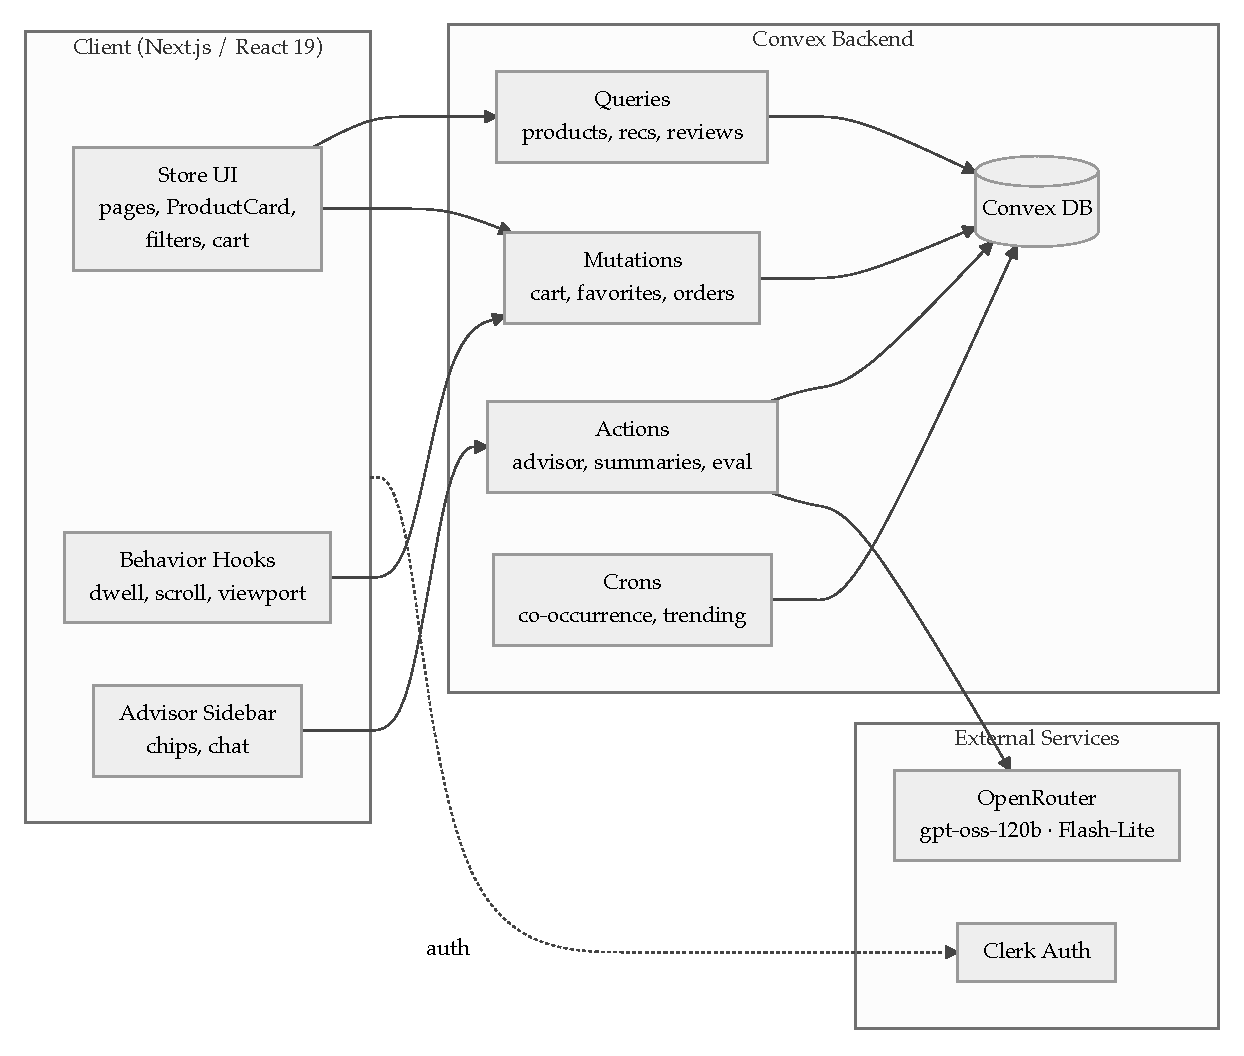
\includegraphics[width=0.95\linewidth]{architecture-overview.pdf}
  \caption{High-level system architecture: Next.js client, Convex
    backend (queries, mutations, actions, crons, database), and
  external services (Clerk and OpenRouter).}
  \label{fig:architecture-overview}
\end{figure}

The client is a Next.js~16 application using React~19 and the
React Compiler. Pages render server-side where possible and
switch to client components only at interaction boundaries.
Tracking hooks, the advisor surface, and behavior aggregation run
on the client. The store catalog is read through Convex reactive
queries, so adding a favorite or seeding a new product propagates
to subscribed components without a manual refetch.

The backend is a single Convex deployment. Convex provides
queries (read-only, reactive, transactional), mutations (write,
transactional), actions (non-transactional, allowed to call
external services), crons, and a TypeScript schema. All
persistent state lives in Convex tables. The seed pipeline runs
as a Convex action, the recommendation cron runs as a Convex
action, and the advisor agent runs as a Convex action with
tool-calling enabled. Convex was chosen over a conventional
REST-plus-SQL-plus-queue stack because the prototype needs
reactive UI updates, scheduled batch flows, and a shared schema
between server and client, and Convex delivers these natively.
The tradeoff is vendor lock-in, accepted at prototype scale.

\section{Codebase and Deployment}
\label{sec:sys-codebase}

The repository is a Turborepo monorepo using bun workspaces:
\texttt{apps/web} (the Next.js frontend),
\texttt{packages/backend} (the Convex backend with
\texttt{convex/ai/} grouping the advisor, prompts, models,
review summaries, and eval integration),
\texttt{packages/ui} (shared design system),
\texttt{packages/eval} (the LLM eval harness),
\texttt{packages/env} (type-safe environment validation), and
\texttt{packages/config} (shared TypeScript configuration). The
eval harness depends on the backend, so scoring runs invoke the
same advisor action as the production client.

The application is deployed on a single VPS. Dokploy orchestrates
four containerized services behind a Traefik reverse proxy (TLS
via Let's Encrypt, hostname-based routing): the Next.js app, the
Convex API origin, the Convex HTTP-actions site, and the Convex
admin dashboard, with the Convex deployment self-hosted against a
co-located Postgres instance. Push-to-main triggers a GitHub
Actions workflow that runs \texttt{convex deploy} in parallel
with Dokploy's auto-deploy of the Next.js Docker image. The
posture is deliberately not hyperscale: the prototype runs on one
VPS and has to run convincingly end to end, not at scale.

\section{Data Layer}
\label{sec:sys-data}

The Convex schema defines twelve tables grouped logically into
four domains: catalog, transactional, behavior-and-AI, and
recommendation precomputation.
Figure~\ref{fig:er-diagram} shows the grouped
entity-relationship view.

\begin{figure}[ht]
  \centering
  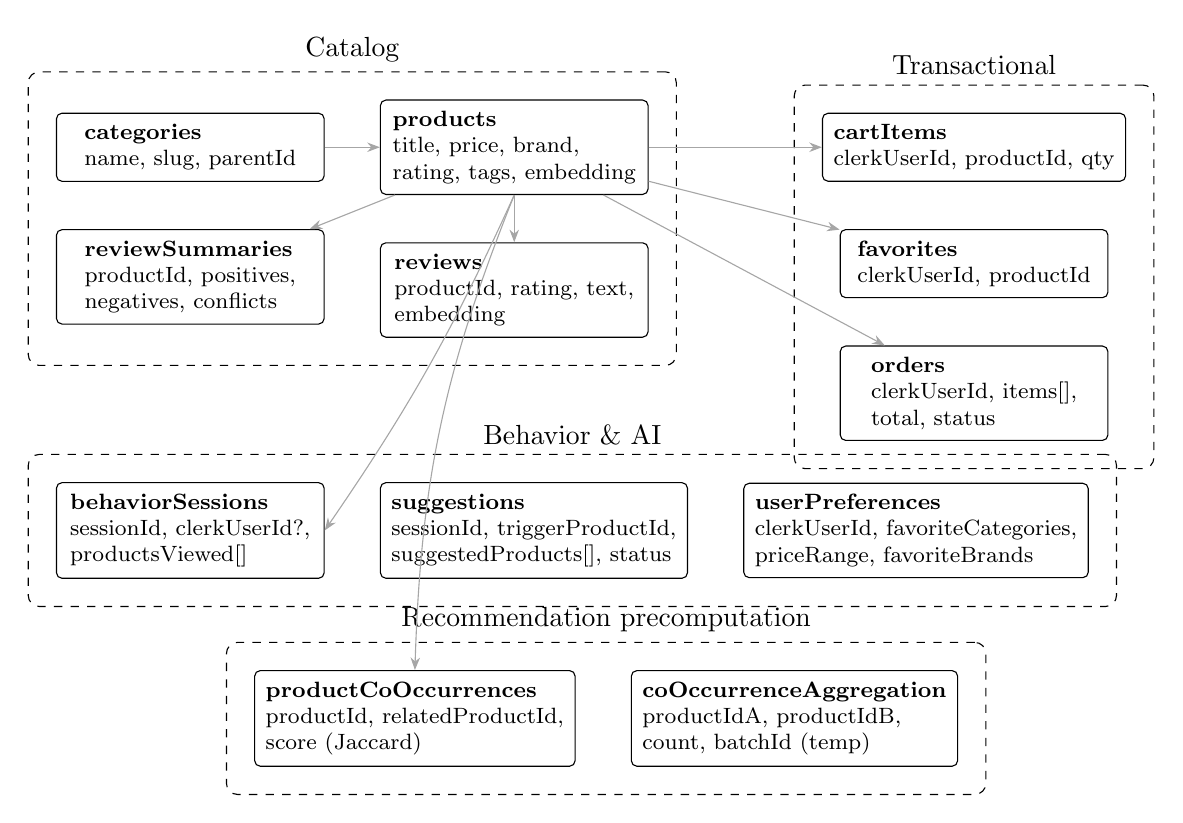
\begin{tikzpicture}[
      node distance=0.6cm and 0.7cm,
      tab/.style={draw, rounded corners=2pt, align=left,
      font=\footnotesize, fill=white, minimum width=3.4cm, inner sep=4pt},
      grp/.style={draw, dashed, rounded corners=4pt, inner sep=10pt,
      font=\small\bfseries},
      rel/.style={-{Stealth[length=1.6mm]}, gray!70, thin}
    ]
    \node[tab] (cat) {\textbf{categories} \\ name, slug, parentId};
    \node[tab, right=of cat] (prod) {\textbf{products} \\ title,
    price, brand, \\ rating, tags, embedding};
    \node[tab, below=of prod] (rev) {\textbf{reviews} \\ productId,
    rating, text, \\ embedding};
    \node[tab, below=of cat] (rsum) {\textbf{reviewSummaries}
    \\ productId, positives, \\ negatives, conflicts};

    \node[grp, fit=(cat)(prod)(rev)(rsum), label={above:Catalog}] (catalog) {};

    \node[tab, right=2.2cm of prod] (cart) {\textbf{cartItems}
    \\ clerkUserId, productId, qty};
    \node[tab, below=of cart] (fav) {\textbf{favorites}
    \\ clerkUserId, productId};
    \node[tab, below=of fav] (ord) {\textbf{orders} \\ clerkUserId,
    items[], \\ total, status};

    \node[grp, fit=(cart)(fav)(ord), label={above:Transactional}] (trans) {};

    \node[tab, below=2.0cm of rsum] (beh) {\textbf{behaviorSessions}
    \\ sessionId, clerkUserId?, \\ productsViewed[]};
    \node[tab, right=of beh] (sug) {\textbf{suggestions}
    \\ sessionId, triggerProductId, \\ suggestedProducts[], status};
    \node[tab, right=of sug] (pref) {\textbf{userPreferences}
    \\ clerkUserId, favoriteCategories, \\ priceRange, favoriteBrands};

    \node[grp, fit=(beh)(sug)(pref), label={above:Behavior \& AI}] (bai) {};

    \node[tab, below=of bai.south, yshift=-0.2cm, xshift=-2.0cm]
    (cooc) {\textbf{productCoOccurrences} \\ productId,
    relatedProductId, \\ score (Jaccard)};
    \node[tab, right=of cooc] (caggr)
    {\textbf{coOccurrenceAggregation} \\ productIdA, productIdB,
    \\ count, batchId (temp)};

    \node[grp, fit=(cooc)(caggr), label={above:Recommendation
    precomputation}] (recg) {};

    \draw[rel] (cat) -- (prod);
    \draw[rel] (prod) -- (rev);
    \draw[rel] (prod) -- (rsum);
    \draw[rel] (prod) -- (cart);
    \draw[rel] (prod) -- (fav);
    \draw[rel] (prod) -- (ord);
    \draw[rel] (prod.south) to[bend right=10] (cooc.north);
    \draw[rel] (prod.south) to[bend left=5] (beh.east);
  \end{tikzpicture}
  \caption{Data model grouped by domain. Foreign keys flow from
    \texttt{products} into the transactional, behavior, and
    recommendation tables. Anonymous behavior sessions carry only
    \texttt{sessionId}; \texttt{clerkUserId} is attached for
  authenticated traffic.}
  \label{fig:er-diagram}
\end{figure}

The \texttt{products} table is denormalized: it stores
\texttt{category} as a string alongside \texttt{categoryId} and
keeps \texttt{rating} and \texttt{reviewCount} on the row. Every
product card render is a single indexed read with no joins, which
is what lets grid pages stream from Convex with no intermediate
compute. The table declares nine indices, each tied to a specific
recommendation-slot query pattern. The \texttt{reviews} table
carries a 3072-dimensional vector index over its embedding field,
which powers the theme-verification path in
Section~\ref{sec:sys-validation}.

\paragraph{Seed pipeline.} The seed runs as a Convex action with
a deterministic faker seed. About 200 products from the
DummyJSON feed are supplemented with faker.js attributes and
enriched with \texttt{useCases} and \texttt{goodFor} fields by a
batch Flash-Lite call modeled on COSMO~\cite{COSMO}. Roughly 50
user personas and 500 orders cluster each persona's history
around its preferences with a power-law spend distribution.
Reviews are AI-generated by a Flash-Lite batch call (20--30
reviews per product, four sentiment profiles, intentional
thematic overlap; about 4\,836 reviews total) so review
summarization has something to summarize.

\section{Recommendation Engine}
\label{sec:sys-recommendations}

The classical recommendation engine implements the four families
formalized in Section~\ref{sec:found-similarity} as a Stage~1
candidate generator. The pipeline lives in two files:
\texttt{convex/recommendations.ts} (Convex queries, mutations,
actions) and \texttt{convex/recommendationHelpers.ts} (pure
TypeScript algorithms with no Convex imports). Splitting the
algorithms from the runtime makes them independently testable.

\paragraph{Co-occurrence with Jaccard.} The
``frequently bought together'' slot reads precomputed Jaccard
scores from the \texttt{productCoOccurrences} table. Computation
runs as a daily cron action that reads all orders, builds the
pair counts and per-product order counts, and emits the
top-$N$ Jaccard-scored neighbors per product. At the seeded scale
(about 500 orders averaging three items each) a single Convex
action recomputes the full top-20-per-product set well under the
action timeout. A minimum-support filter of $\ge 2$
co-occurrences suppresses spurious pairs.

\paragraph{Content-based similarity.}
Listing~\ref{lst:content-similarity} shows the content-similarity
function in full. It is a weighted sum over six attribute
comparisons with the weights from
Section~\ref{sec:found-similarity}. The fact that this is a
12-line function with zero external dependencies is the point: at
the prototype's catalog scale, classical content-based similarity
is trivially cheap and is enough to fill the
``similar products'' slot on every product detail page.

\begin{listing}[ht]
\begin{minted}{typescript}
export function contentSimilarity(
  a: ProductAttrs, b: ProductAttrs, maxPriceRange: number
): number {
  return (
    0.25 * (a.category === b.category ? 1 : 0) +
    0.20 * jaccard(a.tags, b.tags) +
    0.15 * jaccard(a.useCases ?? [], b.useCases ?? []) +
    0.10 * jaccard(a.goodFor ?? [], b.goodFor ?? []) +
    0.10 * (a.brand === b.brand ? 1 : 0) +
    0.10 * priceProximity(a.price, b.price, maxPriceRange) +
    0.10 * ratingProximity(a.rating, b.rating)
  );
}
\end{minted}
  \caption{The content-similarity function. Weights sum to 1.0. The
    \texttt{useCases} and \texttt{goodFor} fields are produced
    once per product during seed via a batch Flash-Lite
    call~\cite{COSMO}, contributing structured similarity that
  pure attribute matching would miss.}
  \label{lst:content-similarity}
\end{listing}

\paragraph{Trending and personalized.} Trending uses the
exponential-decay formula with $\lambda \approx 0.0495$
(14-day half-life). The score is precomputed nightly into the
\texttt{trendingScore} field, so the slot is one indexed read at
query time. Personalized recommendations follow a switching
hybrid keyed on user purchase count, as formalized in
Section~\ref{sec:found-classical}: cold users fall through to
trending, lukewarm users get content similarity to favorites
plus category trending, warm users get a blend of co-occurrence
and content similarity. Signals are combined using Reciprocal
Rank Fusion with $k = 60$, followed by Maximal Marginal
Relevance at $\lambda = 0.7$ to force diversity. The full
hybrid is about 80 lines of straight-line code; no library is
involved.

Figure~\ref{fig:two-stage-pipeline} shows the two-stage pipeline,
connecting the candidate generator described above to the LLM
rerank step in Section~\ref{sec:sys-llm}.

\begin{figure}[ht]
  \centering
  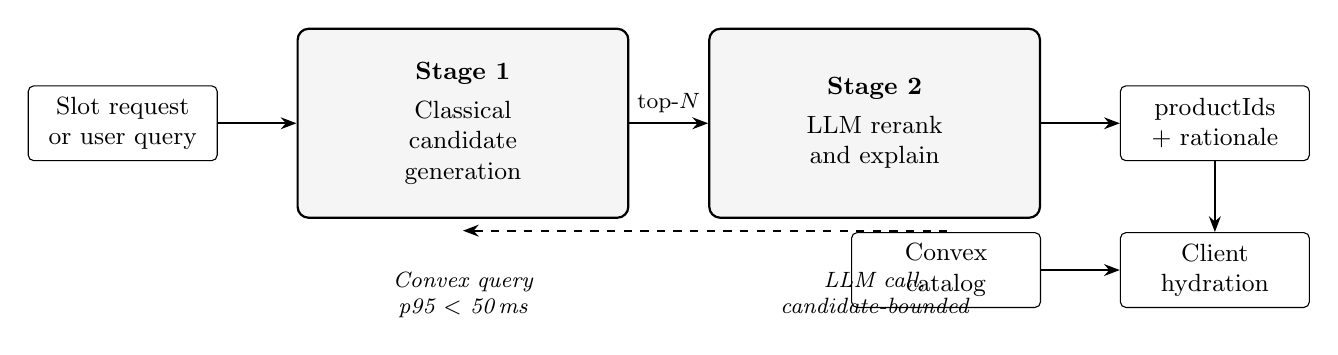
\begin{tikzpicture}[
      box/.style={draw, rounded corners=2pt, align=center, minimum
      width=2.4cm, minimum height=0.95cm, font=\small},
      stage/.style={draw, thick, rounded corners=4pt, align=center,
        minimum width=4.2cm, minimum height=2.4cm,
      font=\small\bfseries, fill=gray!8},
      arr/.style={-{Stealth[length=2mm]}, thick},
      note/.style={font=\footnotesize\itshape, align=center}
    ]
    \node[box] (query) {Slot request \\ or user query};
    \node[stage, right=1.0cm of query] (s1) {Stage~1 \\[3pt]
      \normalfont\small Classical \\ \normalfont\small candidate
    \\ \normalfont\small generation};
    \node[stage, right=1.0cm of s1] (s2) {Stage~2 \\[3pt]
    \normalfont\small LLM rerank \\ \normalfont\small and explain};
    \node[box, right=1.0cm of s2] (out) {productIds \\ + rationale};
    \node[box, below=0.9cm of out] (hyd) {Client \\ hydration};
    \node[box, left=1.0cm of hyd] (db) {Convex \\ catalog};

    \draw[arr] (query) -- (s1);
    \draw[arr] (s1) -- node[above, font=\footnotesize] {top-$N$} (s2);
    \draw[arr] (s2) -- (out);
    \draw[arr] (out) -- (hyd);
    \draw[arr] (db) -- (hyd);
    \draw[arr, dashed] (db.north) |- ([yshift=-0.15cm]s1.south);

    \node[note, below=0.55cm of s1] {Convex query \\ p95 $<$ 50\,ms};
    \node[note, below=0.55cm of s2] {LLM call, \\ candidate-bounded};
  \end{tikzpicture}
  \caption{Two-stage recommendation pipeline. Stage~1 reads the
    catalog and returns a small candidate set. Stage~2 invokes
    the LLM only over that set and emits identifiers plus a
    rationale. Live product fields are hydrated on the client.
    The dashed arrow indicates that Stage~1 reads from the Convex
  catalog; the LLM never reads the catalog directly.}
  \label{fig:two-stage-pipeline}
\end{figure}

\section{Behavior Tracking and Readiness Signals}
\label{sec:sys-behavior}

Behavior tracking is five client-side hooks in
\texttt{apps/web/src/hooks/}. \texttt{useDwellTime} runs a tick
counter while the cursor is over a product container.
\texttt{useViewportTracking} accumulates
IntersectionObserver-reported visible time.
\texttt{useScrollDepth} maintains the page-level maximum scroll
fraction. \texttt{useProductEngagement} composes the first three
behind a single product-scoped facade.
\texttt{useBehaviorTracker} aggregates everything into the
per-session buffer that flushes to the backend.

Listing~\ref{lst:use-dwell-time} shows the core of
\texttt{useDwellTime}. The hook has two effects: one attaches the
\texttt{mouseenter} and \texttt{mouseleave} listeners, and one
runs a 100~ms tick interval while the cursor is hovering. The
cumulative dwell time is the sum of previous hover sessions plus
the current ongoing tick count, which lets the consuming
component read the live value without waiting for a hover to end.

\begin{listing}[ht]
\begin{minted}{typescript}
useEffect(() => {
  if (!element) return;
  const enter = () => setIsHovered(true);
  const leave = () => {
    setIsHovered(false);
    setCurrentMs((prev) => {
      setCumulativeMs((cum) => cum + prev);
      return 0;
    });
  };
  element.addEventListener("mouseenter", enter);
  element.addEventListener("mouseleave", leave);
  return () => {
    element.removeEventListener("mouseenter", enter);
    element.removeEventListener("mouseleave", leave);
  };
}, [element]);
\end{minted}
  \caption{The hover-tracking effect inside \texttt{useDwellTime}.
    Mouse enter and leave listeners are attached imperatively; on
    leave, the in-progress tick total is folded into the
  cumulative dwell value.}
  \label{lst:use-dwell-time}
\end{listing}

\paragraph{Aggregation and flush.}
\texttt{useBehaviorTracker} keeps a
\texttt{Map<productId, TrackedProduct>} buffer plus a
\texttt{ref} mirror so the flush callback reads current state
without triggering a re-render. Aggregation is lossless within
the flush window (maximum dwell, scroll depth, hover time, and
the boolean OR of \texttt{viewedReviews} per product). Three
subscriptions invoke the flush: a 5-second interval, a
pathname-change effect, and a \texttt{visibilitychange} listener
that catches tab close. Convex performs max-value merging on
conflict, so the same session can flush multiple times without
losing aggregate state (Figure~\ref{fig:behavior-flush}).

\begin{figure}[ht]
  \centering
  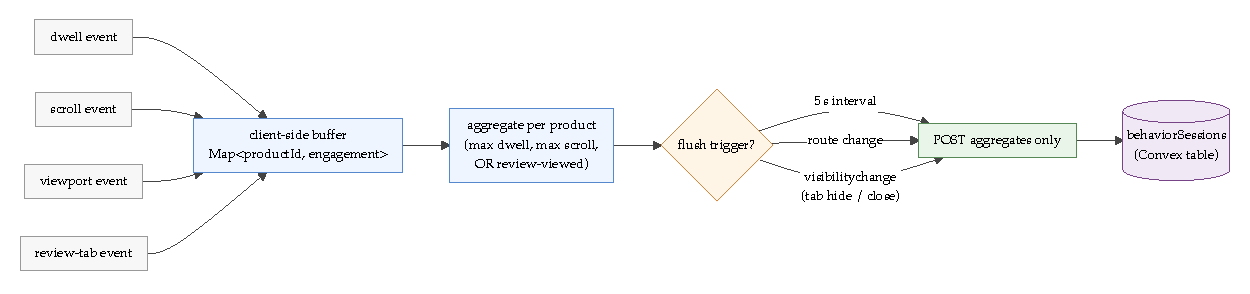
\includegraphics[width=0.88\linewidth]{behavior-flush.pdf}
  \caption{Behavior aggregation and flush pipeline. Events from
    four tracking hooks are buffered per product and flushed on
    a 5-second interval, route change, or tab visibility change,
  sending only aggregate fields to the backend.}
  \label{fig:behavior-flush}
\end{figure}

\paragraph{Readiness signals.} Five signals run continuously on
the client. Each maps to an ambient indicator, not an action.
Product dwell longer than 15~s on a detail page (or 5~s on a
card) and deep scroll past 50\% trigger a breathing animation on
the advisor button. Review-section visibility surfaces a
``What do buyers think?'' chip. Three products viewed in a
category without an add-to-cart surfaces a
``Compare these products?'' chip. Items in the cart during
away-navigation surface a ``Need help deciding?'' chip. The
\texttt{useReadinessSignals} hook reads the in-memory behavior
state and returns \texttt{shouldPulseAdvisor} and
\texttt{activeChips}; dismissed chips persist for the session.
A composite interest score over dwell, scroll, hover, and
review-tab engagement is also computed and kept as a
context-richness hint for the advisor prompt, but the simpler
per-signal thresholds proved more legible during early
dogfooding and are what currently drive the indicators. The
evaluator runs entirely client-side; no LLM call is issued by
this loop.

\section{LLM Advisor}
\label{sec:sys-llm}

The advisor is a Convex action wrapping an instance of
\texttt{@convex-dev/agent}, the official Convex agent component.
The component handles thread persistence, message ordering,
streaming, and AI SDK integration. The application code defines
the model selection, the system prompt, and the tools the agent
can call.

\paragraph{Model routing.} Two tiers from a single provider
(OpenRouter) are used. The conversational tier is
\texttt{openai/gpt-oss-120b}, served by Cerebras with Groq as
fallback, at medium reasoning effort. The batch tier is
\texttt{google/gemini-3.1-flash-lite-preview} with reasoning
disabled. Listing~\ref{lst:select-model} shows
\texttt{selectModel} from \texttt{convex/ai/models.ts}: the model
map resolves a query type to a model identifier, and for gpt-oss
models, provider routing prefers Cerebras then Groq for
throughput.

\begin{listing}[ht]
\begin{minted}{typescript}
const FLASH = "openai/gpt-oss-120b";
const FLASH_LITE = "google/gemini-3.1-flash-lite-preview";

const MODEL_MAP: Record<QueryType, string> = {
  conversational: FLASH,
  comparison: FLASH,
  personalized_advice: FLASH,
  review_summary: FLASH_LITE,
  quick_qa: FLASH_LITE,
  homepage_hero: FLASH_LITE,
};

export function selectModel(queryType: QueryType) {
  const modelId = MODEL_MAP[queryType];
  if (modelId.startsWith("openai/gpt-oss")) {
    return openrouter(modelId, {
      reasoning: { effort: "medium" },
      provider: { order: ["cerebras", "groq"], allow_fallbacks: true,
                  sort: "throughput" },
    });
  }
  return openrouter(modelId);
}
\end{minted}
  \caption{The model-routing function. The \texttt{provider.order}
    array pins Cerebras as the preferred backend for gpt-oss-120b;
    \texttt{allow\_fallbacks} permits OpenRouter to switch to Groq
    if Cerebras is unavailable. The throughput sort matches the
  latency-sensitive nature of the conversational tier.}
  \label{lst:select-model}
\end{listing}

\paragraph{Agent, tools, and prompt.} The agent is constructed
once per cold start as a module-level constant with
\texttt{maxSteps: 12} as the step budget. The value is tuned by
hand: \texttt{gpt-oss-120b} is aggressive with tool calls (three
to five per turn is typical), and an earlier value of 5 caused
the agent to exhaust the budget before producing a final text
answer. That is the failure the eval harness's
\texttt{hasFinalAnswer} scorer was added to catch automatically.
Five tools are registered: \texttt{getProductDetails},
\texttt{searchProducts}, \texttt{getRecommendations} (which
dispatches to similar, frequently-bought-together, or trending),
\texttt{getCartContents}, and \texttt{getReviewsSummary} (which
returns the structured summary including the conflicts list).
Each tool wraps a Zod input schema and an async execute function
via the \texttt{createTool} helper. No tool generates free text
and no tool returns synthesized data: every field is read
directly from the live Convex catalog. This is
hydration-over-generation in action
(Section~\ref{sec:found-grounding}). The system prompt encodes
the design constraints as hard rules (``always use tool results
for factual claims, never guess prices, ratings, or
specifications''; ``never recommend products already in the
customer's cart''; ``when discussing reviews, surface both
positives and negatives with counts; if conflicts exist, always
mention them''). The prompt is the first line of defense; the
validation pipeline in Section~\ref{sec:sys-validation} is the
structural guarantee.

\paragraph{Advisor sidebar UI.} The advisor surface is a
push-content sidebar (page content shifts left instead of being
overlaid by a modal). Four components compose it under
\texttt{components/advisor/}: the floating button with the
breathing animation, the sidebar container, the input composer,
and the message list. Streaming comes from the agent component's
\texttt{useUIMessages} hook, keyed on a thread ID created with a
separate \texttt{createThread} mutation so the client subscribes
before the streaming action begins.
Figure~\ref{fig:advisor-request} traces a single end-to-end
advisor request.

\begin{figure}[ht]
  \centering
  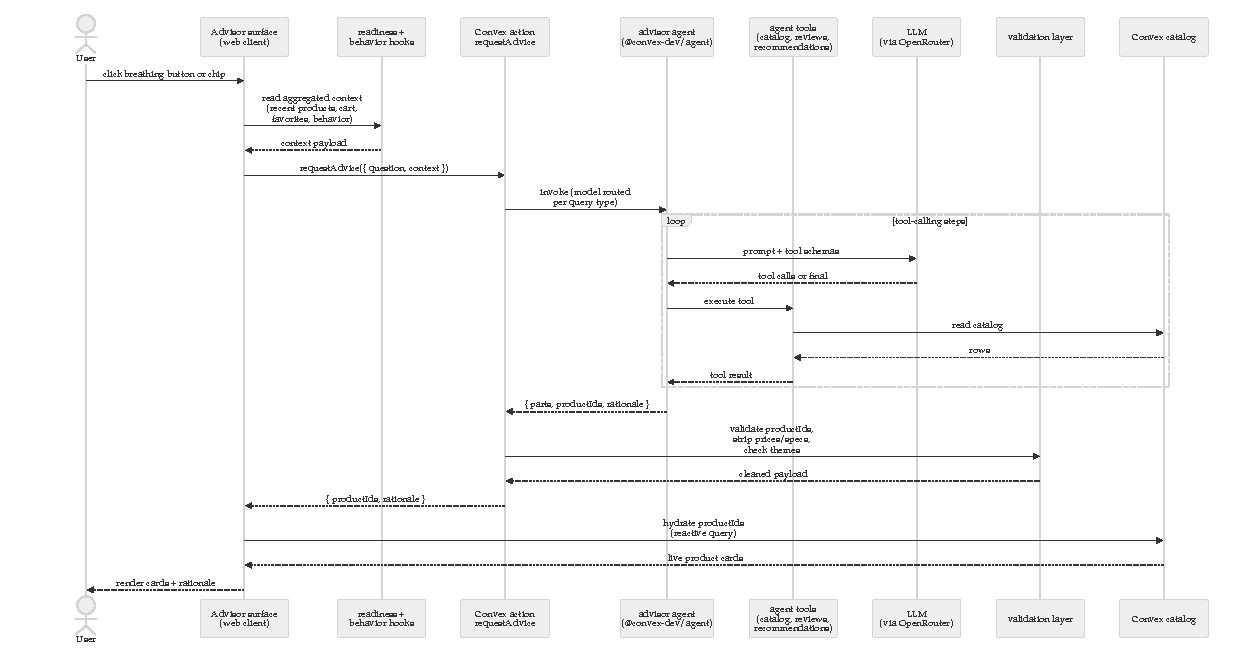
\includegraphics[width=0.92\linewidth]{advisor-request.pdf}
  \caption{End-to-end advisor request. The user click is the
    only entry point. The client assembles context from the
    readiness and behavior hooks. The Convex action invokes the
    agent with a model routed per query type. The agent runs a
    tool-calling loop against the catalog. Validation strips any
    unverifiable claims. The client hydrates the productIds
    against the live catalog and renders. No factual data flows
  from the LLM to the UI directly.}
  \label{fig:advisor-request}
\end{figure}

\section{Review Summarization}
\label{sec:sys-reviews}

Per-product review summaries serve two surfaces: the product
detail page and the advisor. The summary is generated offline,
batch-style, against the actual review corpus. No summary is
ever generated on a user-facing critical path. The structure is
fixed: \emph{what buyers like}, \emph{common complaints},
\emph{best for}, and \emph{conflicting opinions} (explicit
disagreement pairs, each annotated with per-side counts). The
conflict-surfacing structure is the anti-Rufus design choice
from Chapter~\ref{chap:background}: ``45 reviews praise battery
life, 12 reviews call it disappointing'' is more useful than
``most users are happy with the battery''.

The generation flow is a daily Convex cron that finds products
whose summary is stale (missing, or whose review count differs
from the current count, or older than seven days) and
regenerates each. Generation reads the full review corpus,
batches it into a Flash-Lite prompt with a structured JSON
schema, and persists the result; every theme carries a
representative quote and the originating reviewId. After
generation, each theme is verified against the review corpus
using the embedding index on the reviews table: the verifier
embeds the theme text, runs a vector search scoped to the
product, and accepts the theme only if at least one review in
the top-$k$ neighbors clears the cosine-similarity threshold
$\tau$ from Section~\ref{sec:found-grounding}. Failing themes
are dropped before persistence; the \texttt{validationDetails}
field records how many were verified versus dropped.

\section{AI-Assisted Comparison}
\label{sec:sys-comparison}

The comparison flow has no Convex action or agent of its own. It
reuses the advisor entry point with two changes. First, the
request payload includes a \texttt{queryType: "comparison"}
hint, which the action uses to pick the comparison-specific
system prompt variant. Second, the agent is invoked with a
smaller step budget (the comparison flow does not need the
tool-calling depth a freeform conversation does), with the same
five tools registered.

The comparison-specific prompt variant restricts the answer to a
structured tradeoff format, forbids a single-winner verdict, and
refuses comparisons across incompatible categories or duplicate
SKUs. Three structural choices define the surface: the user
picks the products (the system does not), the comparison is
multidimensional across price, specs, ratings, and review
themes, and no winner is named. The user makes the call. This is
a deliberate departure from how most shopping AI handles
comparison; the related-work survey in
Section~\ref{sec:bg-comparison} arrives at the same
recommendation~\cite{ShopifyAgentic,SmashingAgenticUX}. The
structured output renders as a side-by-side table built from the
live catalog using the LLM-emitted productIds, plus a free-text
tradeoff narrative; validation (Section~\ref{sec:sys-validation})
strips price and specification claims from the narrative.

\section{Output Validation Pipeline}
\label{sec:sys-validation}

Output validation is implemented at the boundary between the
agent action and the client response, inside the same Convex
action that wraps the agent invocation. The three validators run
sequentially as formalized in
Section~\ref{sec:found-grounding}. Figure~\ref{fig:validation-pipeline}
shows the pipeline.

\begin{figure}[ht]
  \centering
  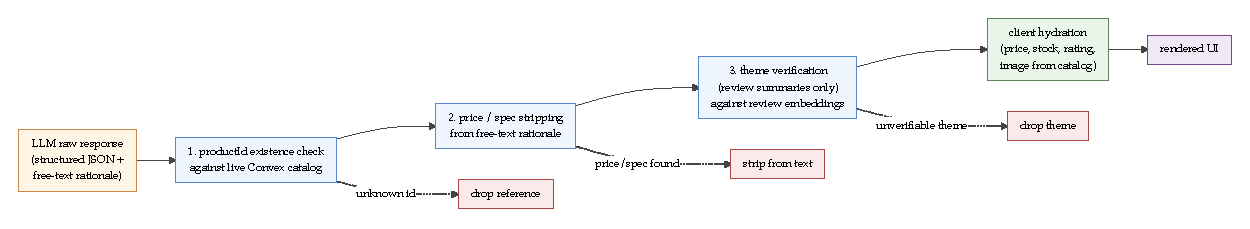
\includegraphics[width=0.94\linewidth]{validation-pipeline.pdf}
  \caption{Output validation pipeline. The structured part of the
    LLM response is checked against the live catalog (productId
    existence). The free-text rationale is scrubbed of price and
    specification claims. Review-summary themes are verified
    against the review corpus before persistence. Failures
  result in dropped references rather than user-visible errors.}
  \label{fig:validation-pipeline}
\end{figure}

\paragraph{Identifier-existence.} Every productId reference the
agent emits is checked against the catalog via a single
\texttt{ctx.runQuery(api.products.get, ...)} per identifier.
Identifiers in $\hat{S} \setminus \mathcal{C}_{id}$ are stripped
from the response before the action returns. The cost is one
indexed read per cited identifier; in practice an advisor turn
cites at most a handful of products, so the latency overhead is
sub-millisecond.

\paragraph{Claim stripping.} The free-text rationale runs
through a small set of regular expressions that match
currency-prefixed numbers, decimal patterns next to keywords
like ``costs'' or ``priced at'', and unit-suffixed numbers near
keywords like ``GB'', ``inches'', ``mAh'', or ``Hz''. Matches
are removed from the rationale. The system prompt already
forbids these claims; the regex pass is the second-line defense
for prompt-following lapses.

\paragraph{Theme verification.} Verification only applies to
outputs that include claimed review themes (the review-summary
surface and certain advisor responses that quote review
feedback). The verifier reuses the embedding-search machinery
from Section~\ref{sec:sys-reviews}: each claimed theme is
embedded, a vector search runs against reviews scoped to the
relevant product, and the theme is dropped if no review in the
top-$k$ clears the similarity threshold.

The three checks are not redundant. Identifier-existence catches
structural hallucinations. Stripping catches drift in free text.
Theme verification catches fabrication in structured outputs
that pass the schema check but are not supported by source data.
Together they encode the design constraint that the LLM is a
candidate selector and a writer, never a source of facts.

\section{Frontend Walkthrough}
\label{sec:sys-frontend}

Two surfaces illustrate the visual contract the system makes
with the user. The first is the homepage with its recommendation
rows. The second is the AI-generated review summary on the
product detail page.

\begin{figure}[ht]
  \centering
  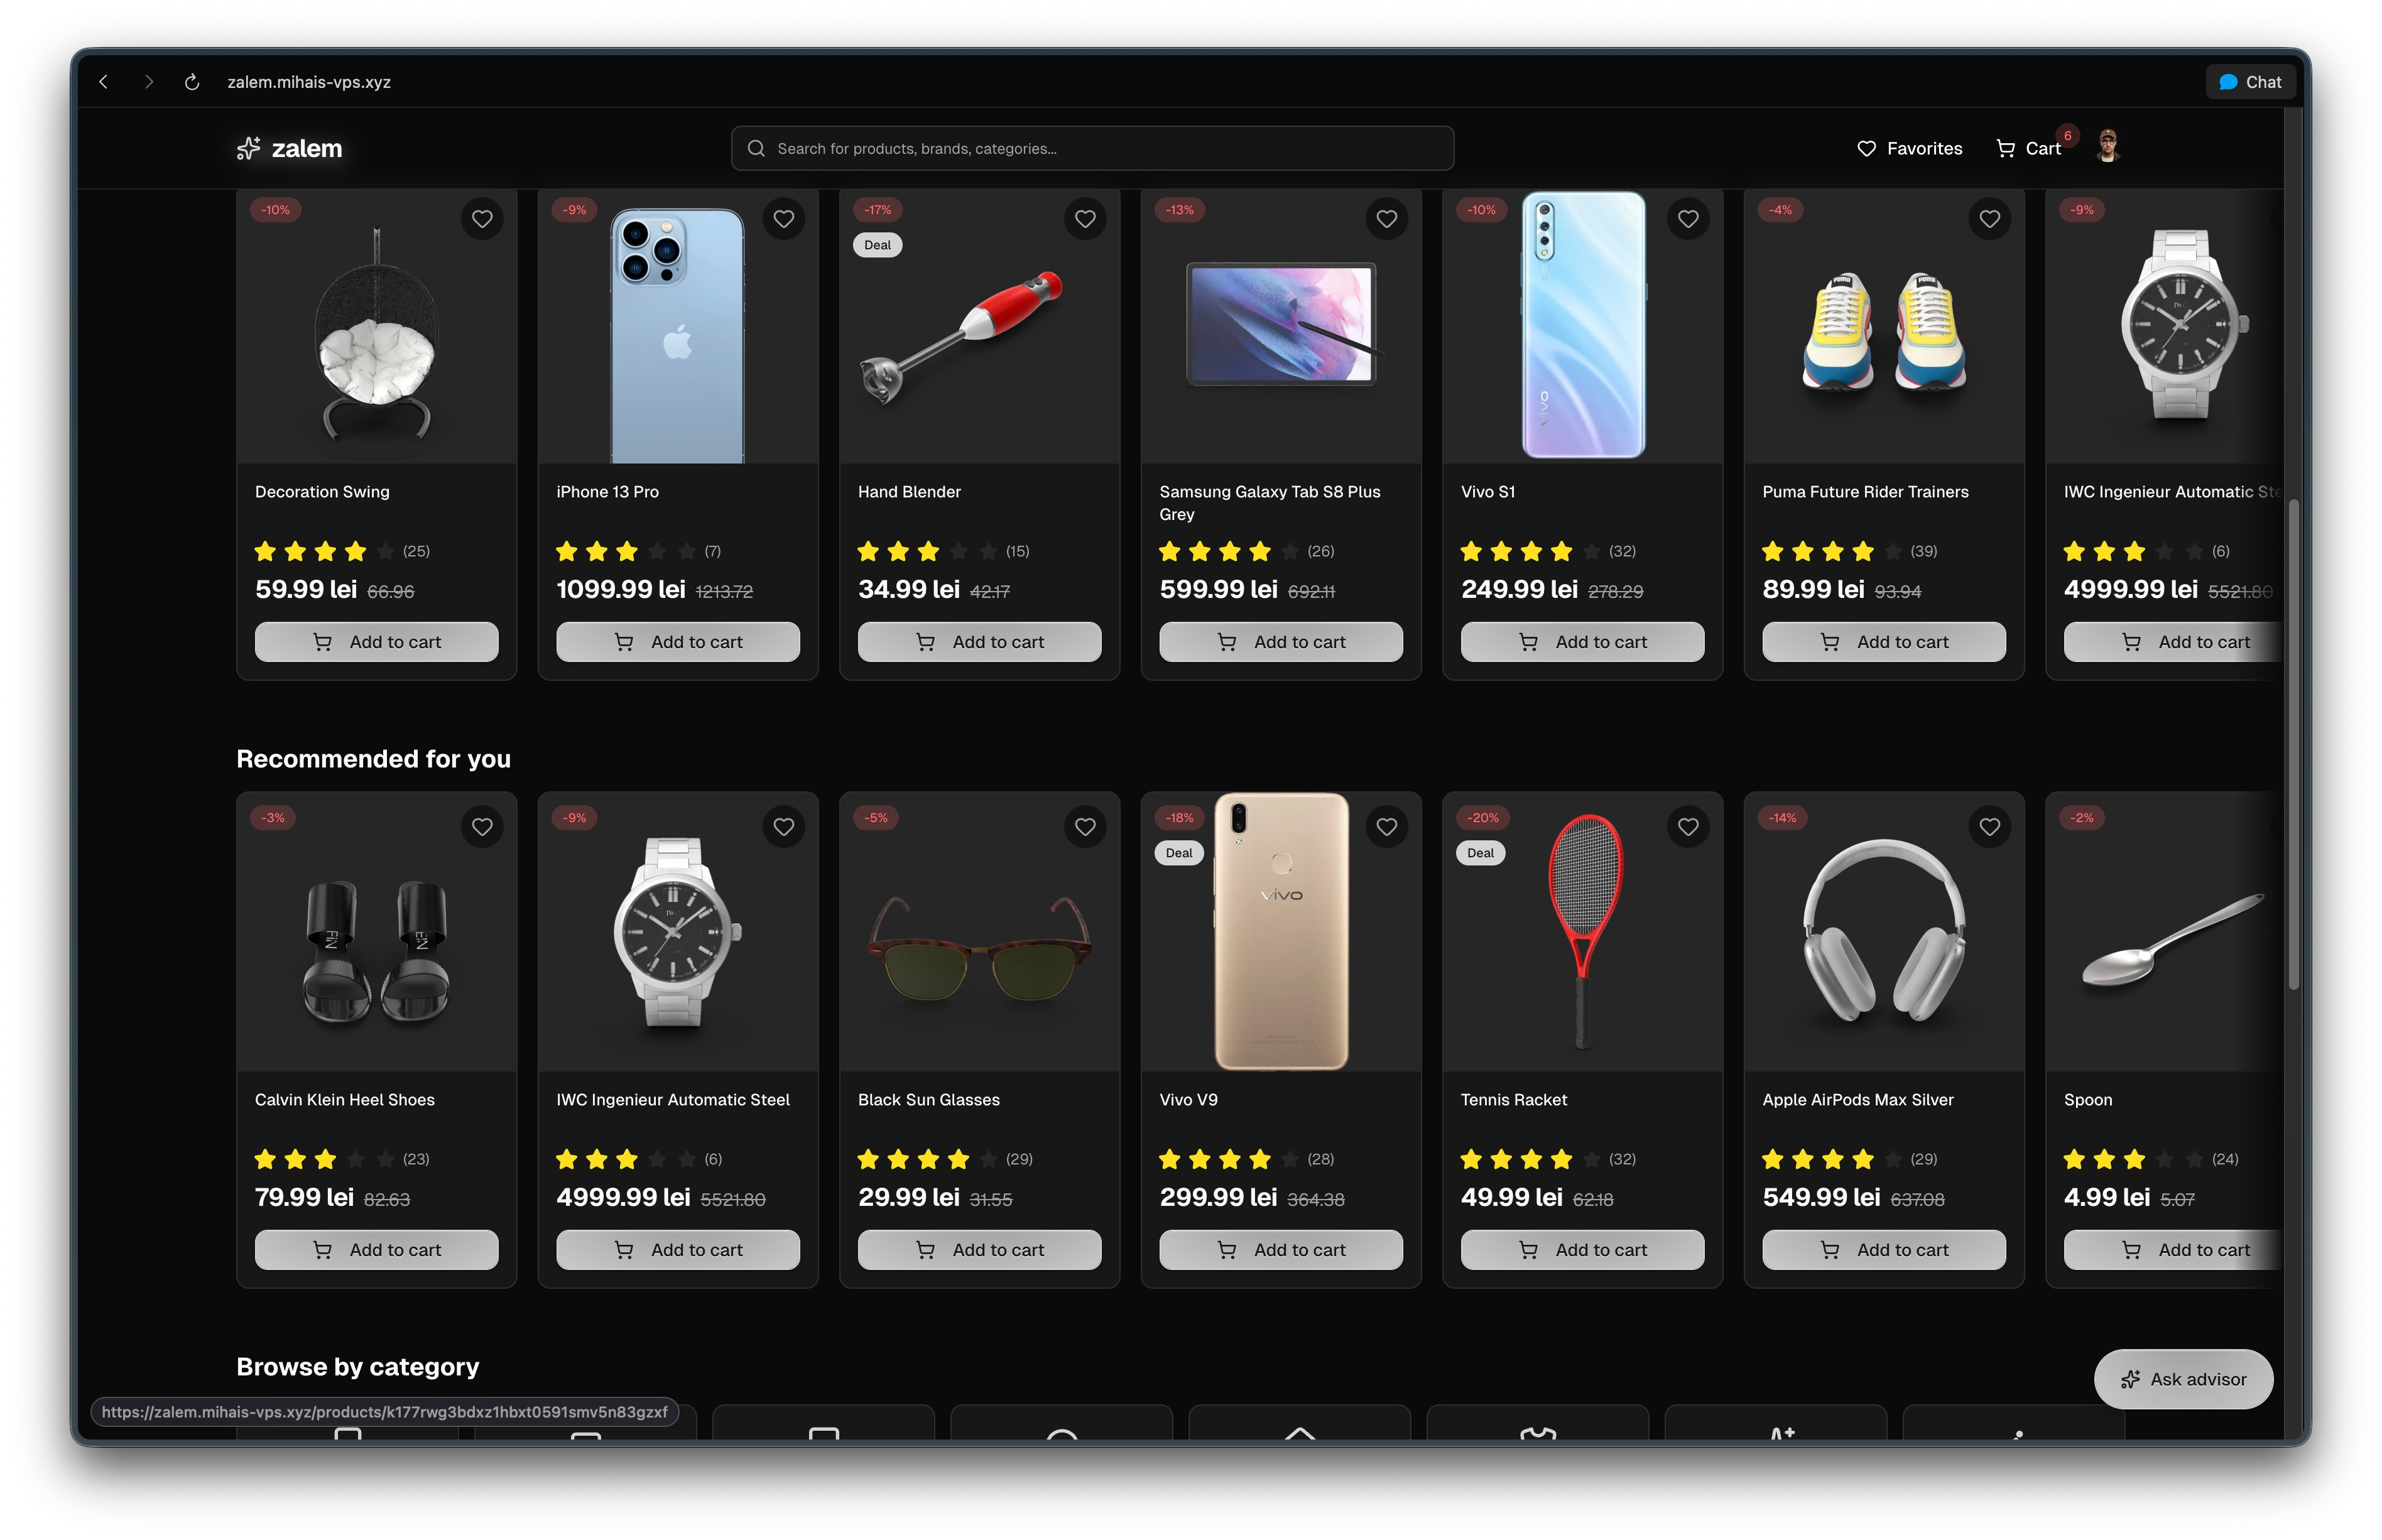
\includegraphics[width=0.95\linewidth]{ui-homepage-recommendations.png}
  \caption{Homepage surface. Two consecutive recommendation rows
    are visible: a popularity-driven row at the top and the
    personalized ``Recommended for you'' row below it. The
    floating advisor button in the lower-right corner is always
  present and idle until a readiness signal fires.}
  \label{fig:ui-homepage}
\end{figure}

The homepage is composed entirely of classical recommendation
slots: a popularity row on top, the personalized
``Recommended for you'' switching-hybrid output below. None of
these invokes an LLM call. The entire homepage renders from
Stage~1. The advisor button in the lower-right corner is idle
until a readiness signal fires, expressing the reactive-first
model visually: the AI is available, never imposed.

\begin{figure}[ht]
  \centering
  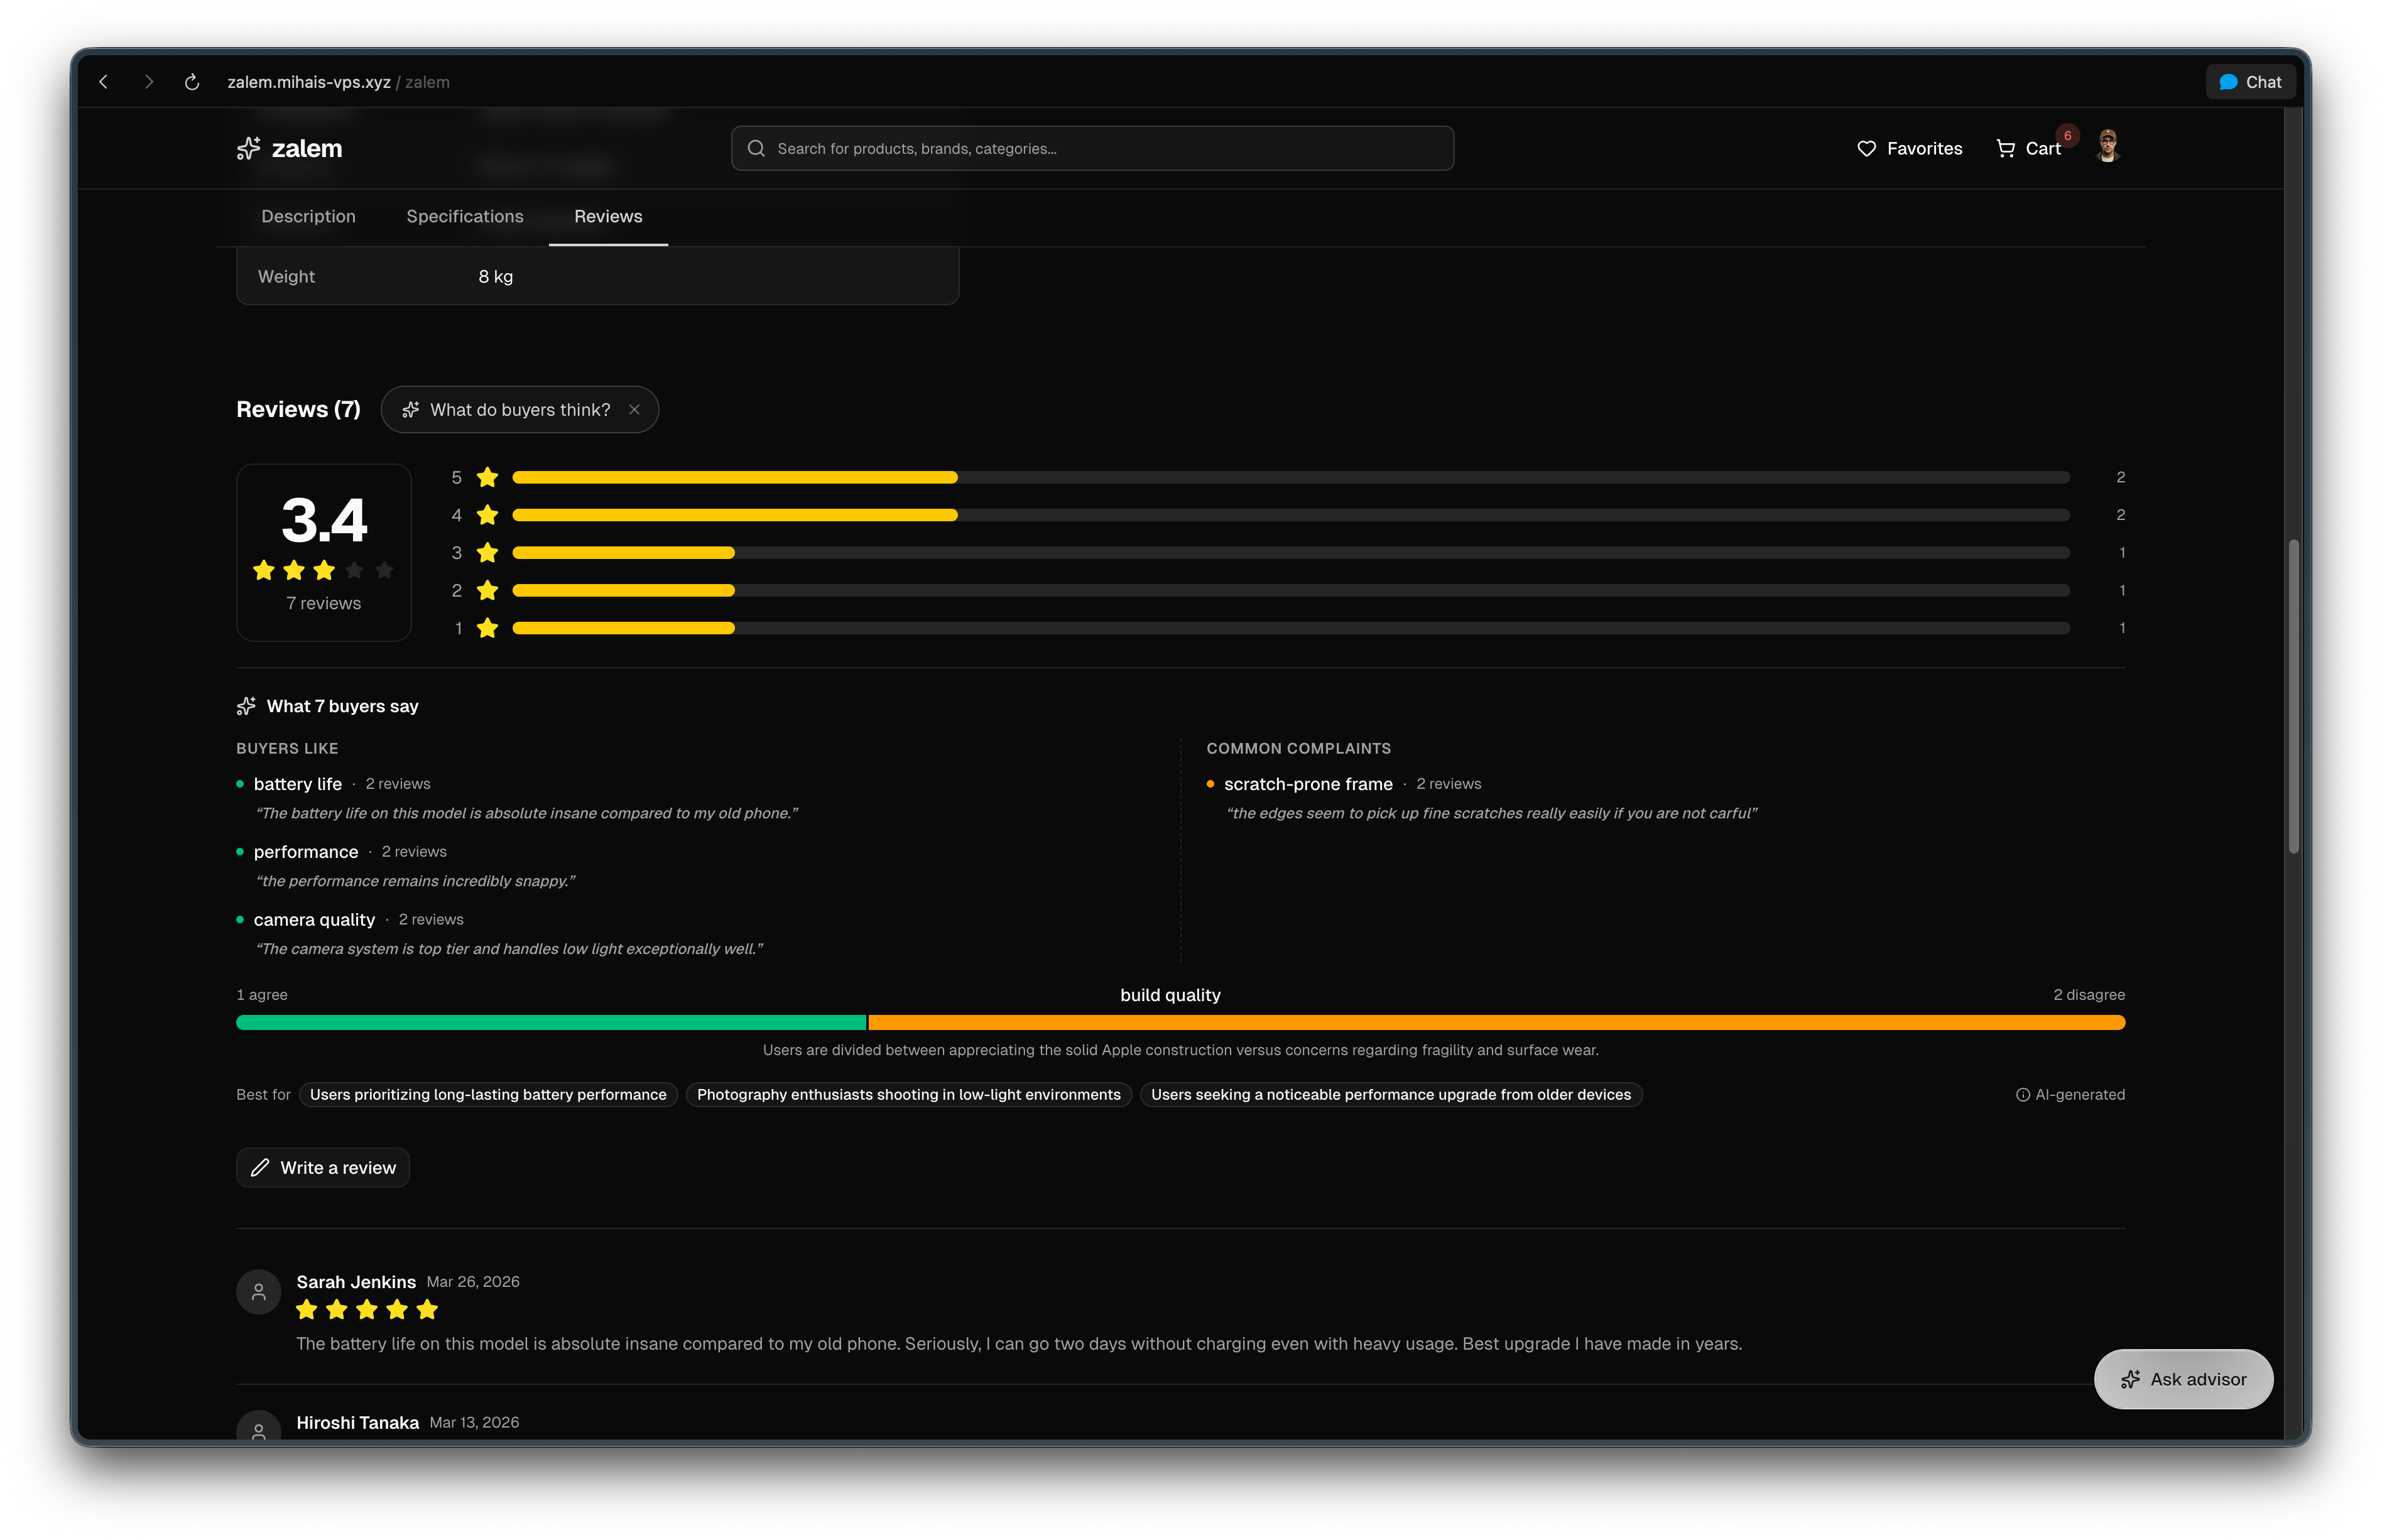
\includegraphics[width=0.95\linewidth]{ui-product-review-summary.png}
  \caption{AI-generated review summary on the product detail
    page. The bipartite conflicts bar surfaces divided opinions
    visually, with per-side counts and a one-sentence
    characterization of each side. The ``Best for'' pills
    surface the structured buyer-cohort field from the summary
  schema. A small ``AI-generated'' tag discloses the synthetic origin.}
  \label{fig:ui-review-summary}
\end{figure}

The review-summary surface concentrates the anti-Rufus design
choices. The explicit positives-and-complaints split shows each
theme with a per-theme count and a representative quote. The
bipartite conflicts bar visualizes divided opinions with
agreeing- and disagreeing-review counts. The ``Best for'' pills
expose the buyer-cohort field. A small ``AI-generated'' tag
discloses the synthetic origin. The contextual
``What do buyers think?'' chip is the review-engagement
readiness signal: it dispatches a question to the advisor on
click but never triggers an LLM call by itself. Neither surface
displays a number, attribute, or price that originates in the
LLM rather than in the live catalog.

\section{Evaluation Harness}
\label{sec:sys-eval}

The eval harness lives in \texttt{packages/eval} and is built
around Promptfoo as the runner with custom shopping-domain
scorers. Section~\ref{sec:found-eval} formalized the scorers and
the composite ranking; this section describes the implementation.
Promptfoo runs the cartesian product of dataset rows and provider
configurations. A custom \texttt{advisorProvider} invokes a
Convex action wrapping the production advisor agent, and
programmatic, built-in, and LLM-as-judge scorers all write into a
single JSON results file per sweep.

\paragraph{Build vs.\ buy.} An honest accounting of where the
engineering effort has thesis value left only the scoring as
distinctive: whether an answer cited a real product, whether a
quoted price matches the database, whether a review theme is
supported by the actual review corpus. These scorers depend on
the live catalog and the embedded review index, and they do not
exist in any off-the-shelf tool. The implementation hands the
generic parts (dataset loading, sweep orchestration, result
storage, local dashboard) to Promptfoo (MIT, open-source) and
ships the shopping-domain scorers as custom JavaScript
assertions.

\paragraph{Dataset.} The dataset is
\texttt{src/datasets/shopping-v1.yaml}, a 25-row YAML file with
each row carrying the question, a simulated context
(\texttt{productId}, \texttt{recentlyViewedIds}), the expected
tools the agent should call, and the productIds the answer
should reference. Rows are distributed across seven categories
(Table~\ref{tab:eval-dataset-categories}). Dataset changes are
versioned by filename, so historical runs are never compared
against new questions.

\begin{table}[ht]
  \centering
  \footnotesize
  \begin{tabular}{|l|c|l|}
    \hline
    \textbf{Category} & \textbf{Rows} & \textbf{What it stresses} \\
    \hline
    simple Q\&A             & 4 & single-tool factual lookup \\
    product validation      & 4 & confirming a single product detail \\
    comparison              & 5 & multi-product tradeoff structure \\
    recommendation          & 5 & switching hybrid + rationale \\
    review summary          & 3 & grounded use of summarized reviews \\
    multi-turn              & 3 & context carryover across turns \\
    edge case               & 1 & ambiguous, off-topic, empty-result \\
    \hline
    \textbf{Total}          & \textbf{25} & \\
    \hline
  \end{tabular}
  \caption{Distribution of dataset rows in
  \texttt{shopping-v1.yaml} across seven categories.}
  \label{tab:eval-dataset-categories}
\end{table}

\paragraph{Configuration sweep.} Nine configurations are
evaluated in the canonical sweep
(Table~\ref{tab:eval-sweep-configs}). The sweep varies four axes:
model identifier, reasoning effort, step budget, and prompt
variant. Promptfoo runs the cartesian product
($9 \times 25 = 225$ advisor invocations).

\begin{table}[ht]
  \centering
  \footnotesize
  \begin{tabular}{|l|l|c|c|l|}
    \hline
    \textbf{Label} & \textbf{Model} & \textbf{Reasoning} &
    \textbf{Steps} & \textbf{Prompt variant} \\
    \hline
    baseline-flash-lite      & gemini-3.1-flash-lite-preview & n/a    & 12 & current \\
    gpt-oss-120b-low         & gpt-oss-120b                  & low    & 12 & current \\
    gpt-oss-120b-medium      & gpt-oss-120b                  & medium & 12 & current \\
    gpt-oss-120b-high        & gpt-oss-120b                  & high   & 12 & current \\
    gpt-oss-20b-low          & gpt-oss-20b                   & low    & 12 & current \\
    gpt-oss-20b-medium       & gpt-oss-20b                   & medium & 12 & current \\
    oss-120b-tight           & gpt-oss-120b                  & medium & 8  & ``be efficient'' \\
    oss-120b-loose           & gpt-oss-120b                  & medium & 15 & current \\
    oss-120b-no-fewshot      & gpt-oss-120b                  & medium & 12 & no few-shot \\
    \hline
  \end{tabular}
  \caption{Configuration sweep for the canonical evaluation.
    Each configuration is run against all 25 dataset rows,
    producing 225 advisor invocations and approximately 1\,125
  LLM-judge calls.}
  \label{tab:eval-sweep-configs}
\end{table}

\paragraph{Scorers.} Five programmatic scorers
(\texttt{hasFinalAnswer}, \texttt{groundedness},
  \texttt{factuality}, \texttt{reviewThemeFidelity},
\texttt{toolCallEfficiency}) plus Promptfoo's built-in
\texttt{tool-call-f1} are registered. Listing~\ref{lst:groundedness}
shows \texttt{groundedness.ts} in full. It is the scorer most
directly aimed at the Rufus 32\% accuracy failure mode.

\begin{listing}[ht]
\begin{minted}{typescript}
const PRODUCT_ID_REGEX = /\bk[0-9a-z]{31}\b/g;

export default async function groundedness(output: string, _ctx: Context) {
  const cited = Array.from(new Set(output.match(PRODUCT_ID_REGEX) ?? []));
  if (cited.length === 0) {
    return { pass: true, score: 1, reason: "vacuously grounded" };
  }
  const lookups = await Promise.all(cited.map(async (id) => {
    try {
      const product = await convex.query(productGetRef, { id });
      return { id, exists: product !== null };
    } catch { return { id, exists: false }; }
  }));
  const missing = lookups.filter((l) => !l.exists).map((l) => l.id);
  const grounded = cited.length - missing.length;
  return {
    pass: missing.length === 0,
    score: grounded / cited.length,
    reason: missing.length === 0
      ? `all ${cited.length} cited productIds exist`
      : `${missing.length}/${cited.length} hallucinated: ${missing.join(", ")}`,
  };
}
\end{minted}
  \caption{The \texttt{groundedness} scorer. Convex IDs are
    32-character URL-safe alphanumerics; products start with a
    lowercase ``k''. Every cited identifier is looked up against
    the live catalog through a typed Convex client. A perfect
  score requires every cited identifier to exist.}
  \label{lst:groundedness}
\end{listing}

Five LLM-as-judge rubrics (completeness, helpfulness, tradeoff
surfacing, tool appropriateness, tone) run on a 0--5 scale with
Claude Haiku~4.5 as the judge model, chosen across model families
to mitigate self-preference bias as formalized in
Section~\ref{sec:found-eval}.

\section{Results}
\label{sec:sys-results}

This section reports the measured findings from the canonical
sweep. The composite score combines judge quality (weight 0.30),
programmatic correctness (0.25), per-query dollar cost (0.20),
p95 latency (0.15), and tool-step efficiency (0.10); cost and
latency enter with negative weight and a per-dimension normalizer
so the composite stays in $[0,1]$. Every configuration ran the
full 34 rows of the dataset (25 questions plus four-rubric judge
invocations), so row coverage is uniform across cells.

\subsection{Ranked Configurations}
\label{subsec:results-sweep}

Table~\ref{tab:results-ranked-configs} reports the ranking.

\begin{table}[ht]
  \centering
  \footnotesize
  % generated by packages/eval/src/reports/thesisExport.ts — do not edit by hand
\begin{tabular}{rlrrrrrr}
\toprule
\# & configuration & quality & correctness & efficiency & avg cost & p95 latency (ms) & composite \\
\midrule
1 & gemini-3.1-flash-lite-preview · none · ms12 · current & 0.776 & 0.941 & 0.515 & \$0.0003 & 4216 & \textbf{0.807} \\
2 & gpt-oss-120b · low · ms12 · current & 0.775 & 0.922 & 0.515 & \$0.0006 & 4705 & \textbf{0.795} \\
3 & gpt-oss-120b · medium · ms12 · no-fewshot & 0.815 & 0.921 & 0.497 & \$0.0006 & 5889 & \textbf{0.774} \\
4 & gpt-oss-20b · medium · ms12 · current & 0.672 & 0.920 & 0.506 & \$0.0005 & 4181 & \textbf{0.768} \\
5 & gpt-oss-120b · medium · ms8 · be-efficient & 0.703 & 0.932 & 0.497 & \$0.0007 & 5734 & \textbf{0.719} \\
6 & gpt-oss-120b · medium · ms15 · current & 0.726 & 0.930 & 0.479 & \$0.0007 & 7466 & \textbf{0.683} \\
7 & gpt-oss-120b · medium · ms12 · current & 0.764 & 0.924 & 0.485 & \$0.0007 & 6053 & \textbf{0.680} \\
8 & gpt-oss-120b · high · ms12 · current & 0.734 & 0.900 & 0.467 & \$0.0010 & 12072 & \textbf{0.492} \\
\bottomrule
\end{tabular}

  \caption{Configurations ranked by composite score. Each row is
    a single configuration evaluated against the 25 rows of
  \texttt{shopping-v1.yaml}.}
  \label{tab:results-ranked-configs}
\end{table}

Three observations follow. The Gemini~3.1 Flash-Lite baseline
ranks \#1 on composite (0.807) despite being treated by the
original design as a cheaper fallback. It loses on raw quality
by 3.9 points to \texttt{no-fewshot} \texttt{gpt-oss-120b}
(0.776 vs.\ 0.815) but wins decisively on both penalty axes:
\$0.0003 per query versus \$0.0005--0.0010, and 4.2~s p95
versus 4.2--12.1~s. Second, \texttt{gpt-oss-120b} at \emph{low}
reasoning ranks \#2 (0.795), and \texttt{no-fewshot} ranks \#3
(0.774) while still producing the highest raw quality in the
sweep. Two things follow: the few-shot examples in the
production prompt are a net negative on this dataset
(Section~\ref{subsec:results-prompt-variant}), and the default
\texttt{medium} reasoning setting is not the composite-optimal
one. Third, raising reasoning effort and loosening the step
budget both hurt the composite uniformly:
\texttt{gpt-oss-120b} high-reasoning is the worst at 0.492
despite competitive raw quality (cost doubles, p95 inflates to
12.1~s), and \texttt{ms15} comes in at 0.683 with raw quality
\emph{below} the \texttt{ms12} default (the extra steps did not
improve the answer).

\subsection{Pareto Fronts}
\label{subsec:results-pareto}

Figures~\ref{fig:results-pareto-cost-quality}
and~\ref{fig:results-pareto-latency-quality} plot each sweep cell
on the (cost, quality) and (latency, quality) planes.

\begin{figure}[ht]
  \centering
  \input{figures/eval-pareto-cost-quality}
  \caption{Cost-quality pareto plot. $x$-axis is average
    per-query cost in USD, $y$-axis is the LLM-judge mean
    quality. Flash-Lite (leftmost) and \texttt{no-fewshot}
  (topmost) are the two non-dominated configurations.}
  \label{fig:results-pareto-cost-quality}
\end{figure}

\begin{figure}[ht]
  \centering
  % generated by thesisExport.ts — do not edit by hand
% requires: \usepackage{pgfplots}
\begin{tikzpicture}
  \begin{axis}[
    width=\linewidth,
    height=8cm,
    xlabel={Average latency (ms)},
    ylabel={Quality (LLM-judge mean)},
    grid=both,
    nodes near coords,
    nodes near coords align={vertical},
    every node near coord/.append style={font=\tiny}
  ]
    \addplot+[only marks, mark=*, point meta=explicit symbolic]
      table[col sep=comma, x=latency, y=quality, meta=label] {eval-pareto-latency-quality.csv};
  \end{axis}
\end{tikzpicture}

  \caption{Latency-quality pareto plot. Flash-Lite anchors the
    low-latency end at competitive quality; \texttt{no-fewshot}
  anchors the high-quality end at moderately higher latency.}
  \label{fig:results-pareto-latency-quality}
\end{figure}

On the cost-quality plane, only two configurations sit on the
frontier. Flash-Lite is unbeaten on cost at the price of 3.9
quality points; \texttt{no-fewshot} is unbeaten on quality at
the price of roughly doubling per-query cost. Every other
configuration lies in the strictly-dominated interior. The
implication for production is that the choice between
Flash-Lite and \texttt{no-fewshot} is the only choice that has
to be made on this evidence. The latency-quality plane tells
the same structural story. Flash-Lite and \texttt{no-fewshot}
again anchor the frontier, with Flash-Lite cheaper \emph{and}
faster (4.2~s p95 versus 5.9~s) at the cost of those 3.9
quality points.

\subsection{Per-Category Programmatic Correctness}
\label{subsec:results-per-category}

Table~\ref{tab:results-per-category} reports per-cell
programmatic-correctness means (averaged across the six
deterministic scorers) restricted to the three categories with
enough rows to support a breakdown.

\begin{table}[ht]
  \centering
  \footnotesize
  % generated by thesisExport.ts — do not edit by hand
\begin{tabular}{lrrrrrr}
\toprule
configuration & comparison & edge\_case & product\_validation & recommendation & review\_summary & simple\_qa \\
\midrule
gemini-3.1-flash-lite-preview · none · ms12 · current & 0.95 & 1.00 & 0.97 & 0.89 & 0.93 & 0.98 \\
gpt-oss-120b · low · ms12 · current & 0.91 & 1.00 & 0.95 & 0.84 & 1.00 & 1.00 \\
gpt-oss-120b · medium · ms12 · no-fewshot & 0.91 & 1.00 & 0.94 & 0.81 & 1.00 & 1.00 \\
gpt-oss-20b · medium · ms12 · current & 0.94 & 1.00 & 0.91 & 0.85 & 1.00 & 0.97 \\
gpt-oss-120b · medium · ms8 · be-efficient & 0.92 & 1.00 & 0.95 & 0.90 & 0.97 & 0.96 \\
gpt-oss-120b · medium · ms15 · current & 0.91 & 1.00 & 0.94 & 0.82 & 0.97 & 1.00 \\
gpt-oss-120b · medium · ms12 · current & 0.93 & 1.00 & 0.91 & 0.83 & 0.97 & 0.99 \\
gpt-oss-120b · high · ms12 · current & 0.92 & 1.00 & 0.89 & 0.79 & 0.85 & 0.94 \\
\bottomrule
\end{tabular}

  \caption{Mean programmatic correctness per category, per
    configuration. Values are bounded in $[0,1]$, higher is
  better.}
  \label{tab:results-per-category}
\end{table}

Programmatic correctness is uniformly high on \texttt{simple\_qa}
(0.94--1.00): when the question is a single factual lookup,
every configuration calls the right tool, the right product
exists, and the price and rating match. This is the floor the
catalog-hydration design is meant to enforce, and the harness
confirms it. \texttt{Recommendation} is where configurations
actually differ, ranging from 0.79 (high-reasoning) to 0.90
(\texttt{ms8} \texttt{be-efficient}). That category is the
structurally hardest case (open-ended candidate ranking,
tradeoff language, no single ground-truth product), and the one
where future dataset growth would produce the most discriminating
signal.

\subsection{Few-Shot Contamination}
\label{subsec:results-prompt-variant}

The harness was built to surface failure modes that the
production UI hides. The cleanest example is the few-shot
contamination the prompt-variant A/B revealed. With the
production prompt (\texttt{gpt-oss-120b}, medium reasoning,
12-step budget, few-shot examples included), the advisor's
responses on simple, ambiguous questions systematically
reference products from the few-shot examples (Logitech~K380
keyboard, Samsung Galaxy~S24~Ultra, iPhone~15~Pro) instead of
the product carried in the row's system context. Removing the
few-shot examples eliminates the contamination.

The qualitative form is clearest on a single row. The dataset
row asks for the price of a Vivo~V9; the row's system context
names the product explicitly.

\begin{quote}
\textbf{\texttt{current} (few-shots included).} ``I'm happy to
look up the price and any current promotions, but could you let
me know which phone you're referring to? \emph{Samsung Galaxy
S24 Ultra}, \emph{iPhone 15 Pro}, or one of the other models
you've been browsing\ldots''

\medskip

\textbf{\texttt{no-fewshot}.} ``The Vivo V9 is priced at
\$299.99. At the moment there's no discount listed for this
model. If a promotion becomes available, it would be reflected
on the product page.''
\end{quote}

The mechanism is mechanical: few-shot examples are injected into
the model's \texttt{messages} array as JSON-encoded
\texttt{user} and \texttt{assistant} turns. On a short ambiguous
query like ``what's the price of this phone?'' the model treats
those turns as recent conversation history and pattern-matches
against the example products instead of the system-context
product. The production UI largely side-steps the failure
because real users arrive with specific questions (from
comparison chips, review-summary buttons), but the harness's
broader query distribution surfaces it. Programmatic and judge
measurements agree on direction: \texttt{no-fewshot} hits the
highest raw judge quality (0.815 vs.\ 0.764 for the
otherwise-identical \texttt{current}) while keeping correctness
within 0.3~pp, and a focused two-configuration A/B from earlier
development ranked the variants identically on all four judge
rubrics. Two scoring methodologies converging on the same
ordinal is what argues the finding is not an artifact of either.

\subsection{Summary and Validity}
\label{subsec:results-summary}

The evidence supports the central claim on two of three axes:
every configuration completes well under the
consumer-tolerance latency bound and at well under one cent per
query, with grounded output across the sweep
(\texttt{groundedness} mean $\ge 0.89$). The harness adds a
finding the claim did not anticipate: a non-trivial design
space exists \emph{within} those bounds where the right choice
is cheaper and less computationally aggressive rather than the
one with the highest raw quality. Higher reasoning effort and
looser step budgets are uniformly worse on composite, which
disproves the implicit ``more reasoning is always better''
assumption. Three validity classes qualify these numbers.
\emph{Internal}: seeded reviews are AI-generated, and residual
judge bias remains despite the cross-family judge choice.
\emph{Construct}: groundedness verifies existence not relevance,
factuality verifies values not semantic correctness, theme
fidelity verifies embedding match not salience. The composite
is reported alongside the pareto fronts, so disagreement with
the weights is recoverable. \emph{External}: 200 products on a
development-tier deployment do not predict 10\,000-product
production load, and the 25-row dataset cannot cover every
failure mode. The methodological finding (programmatic and
cross-family judges agree on ordinal) argues the harness
produces a robust ranking even when individual scorers are
imperfect.

\section{Engineering Challenges}
\label{sec:sys-engineering}

Six engineering challenges hit during implementation justify
choices that affect the metrics above. Each is documented at
length in \texttt{docs/lessons-learned.md}.

\begin{itemize}
  \item \textbf{Hooks before returns.} Every React hook appears
    before any conditional control flow; rules-of-hooks
    violations are caught by strict mode and the React Compiler.
  \item \textbf{Hydration mismatches with Base UI.} Components
    are gated by a \texttt{useMounted} hook implemented with
    \texttt{useSyncExternalStore} (\texttt{getServerSnapshot:
      () => false}), collapsing the typical two-render pattern
    into one.
  \item \textbf{Convex action abort.}
    \texttt{useAction} does not support abort signals; the
    advisor stop button clears the UI loading state but the
    server-side action runs to completion (cost acknowledged in
    the per-turn token figures).
  \item \textbf{\texttt{useUIMessages} typing.}
    \texttt{UIMessagesQueryResult<typeof
      api.ai.queries.listMessages>} derives the message type
    from the source of truth instead of duplicating it.
  \item \textbf{\texttt{content-visibility} grid
    virtualization.} CSS-native
    \texttt{content-visibility: auto} with
    \texttt{contain-intrinsic-size} for 50--150-card grids,
    avoiding any JavaScript virtualizer.
  \item \textbf{100~ms tracking-hook intervals.} Per-element
    intervals are cheap on desktop hardware; potentially
    measurable on low-end mobile.
\end{itemize}

\chapter{Conclusions and Future Work}
\label{chap:conclusions}

\section{Summary}
\label{sec:concl-summary}

AI shopping assistants have moved from research to production at
hyperscale. The published evidence on the largest deployment
documents systematic failures in recommendation accuracy, factual
correctness, and intrusiveness. The question behind this thesis
was whether those failures are inherent to the AI-shopping
problem or whether they come from integration choices a
different system could have made differently. This thesis argues
for the second reading and builds a prototype that shows it.

The prototype combines a two-stage recommendation pipeline
(classical candidate generation followed by LLM rerank and
explanation), a reactive-first advisor surface driven by
lightweight behavior signals, a review-summarization module
grounded in real review text with explicit conflict surfacing,
an AI-assisted comparison flow with no winner verdict, and an
output-validation layer that strips claims the model could
fabricate from free text and checks every cited identifier
against the live catalog.
A custom evaluation harness sits alongside the prototype. It
scores configurations on grounded quality, latency, and cost
across a canonical eight-configuration sweep.

The measured evidence supports the central claim on two of three
axes. Seven of eight configurations stay within a p95 latency of
7.5~s; only \texttt{gpt-oss-120b} at high reasoning effort
rises to 12.1~s. Every configuration costs well under one cent
per query and produces grounded output across the sweep
(\texttt{groundedness} mean $\ge 0.89$ for every configuration).
The harness adds a finding the claim did not anticipate: within
those bounds there is a real design space where the right choice
is the cheaper, lighter configuration, not the one with the
highest raw quality. Higher reasoning
effort and looser step budgets are uniformly worse on composite.
This disproves the implicit ``more reasoning is always better''
assumption that production code tends to encode.

\section{Practical Implications}
\label{sec:concl-implications}

Five recommendations follow from the design and the measured
results.

\begin{description}
  \item[Never let the LLM generate factual product data.]
    Hydration-over-generation reduces the price-hallucination
    surface to zero by construction. Cited identifiers are
    verified against the live catalog; price and specification
    claims are stripped from free text before render.
  \item[Surface review conflicts explicitly with counts.] A
    summary that hides the dissenting minority gives the
    wrong opinion when the minority is large enough to matter;
    the explicit-count format makes that minority visible.
  \item[Keep AI advice user-initiated.] Behavior signals prepare
    context but do not auto-fire the LLM. The reactive surface
    respects user agency and avoids the intrusiveness pattern
    documented for comparable production systems.
  \item[Route by query type.] The harness shows a real
    cost-quality tradeoff between Flash-Lite and
    \texttt{no-fewshot} \texttt{gpt-oss-120b}, and a uniform
    loss from higher reasoning effort. Configuration choices
    should be backed by measured evidence, not intuition.
  \item[Measure every configuration choice.] The few-shot
    contamination finding is the clearest example: the
    production UI hid the failure mode, and only a harness
    running against a broader query distribution surfaced it.
\end{description}

\section{Limitations}
\label{sec:concl-limitations}

The biggest scope limits are the lack of a human-subject
evaluation, the lack of an offline-IR comparison for the
classical recommendation algorithms, the seeded-catalog scale
(about 200 products, 4\,836 AI-generated reviews), and
replication against only a single deployment. The thesis does
not claim to address any of these. It claims that the
engineering work it does report holds up under measurement
within those limits.

\section{Future Work}
\label{sec:concl-future}

A within-subjects user study (perceived usefulness, trust,
intrusiveness, purchase confidence) is the most valuable
extension: the engineering-quality metrics in
Chapter~\ref{chap:system} do not predict UX outcomes, and human
evaluation would close that gap. Adding offline
recommender-quality metrics (Hit~Rate@5, NDCG@10, catalog
coverage, intra-list diversity, popularity-bias Gini) against a
held-out temporal split of the seeded order data is a low-risk
extension that closes the second methodological gap, because it
shares the same data pipeline. Extending the harness to
multi-category catalogs and non-electronics domains would test
whether the theme-fidelity scorer and the comparison flow
generalize beyond the curated dataset. Richer behavior signals
(mouse trajectory, eye tracking, repeated-visit patterns) are
cheap to capture and worth evaluating once human-subject data is
available. Production hardening at 10\,000+ products and traffic
load is documented in \code{docs/scale-considerations.md}.
Turning the eval harness into a CI regression gate with Pareto
comparison against a reference run would let the design
discipline this thesis argues for survive in a real engineering
workflow.

\section{Closing Remarks}
\label{sec:concl-closing}

The thesis argues, end to end, that trustworthy AI shopping
assistance is a problem of integration discipline, not of model
capability. The failure modes documented for the largest
production system can be addressed through structural decisions
a different system can make differently. A working prototype
plus an evaluation harness are enough to show that those
decisions hold up under measurement.


\bibliography{references}

\end{document}
